\chapter[CA sobre imágenes OLCI basada en BLRs]{Corrección atmosférica de imágenes OLCI sobre aguas turbias basada en las bandas roja, NIR y SWIR y una técnica de Residuos de Líneas de Base (BLR)}
\label{blr}

% , un enfoque común para la corrección atmosférica píxel a píxel de las imágenes satelitales de color del mar es calcular las reflectancias del agua y de aerosoles en dos bandas espectrales, típicamente en el infrarrojo cercano (NIR, 700-1000 nm) o en el infrarrojo de onda corta (SWIR, 1000-3000 nm), y luego extrapolar la reflectancia de aerosoles a longitudes de onda más cortas. Para aguas claras, esto se puede lograr simplemente utilizando las bandas NIR, donde la reflectancia del agua se puede suponer insignificante, es decir, el supuesto de \textit{agua negra} (o \textit{píxel negro}, cf. \S \ref{int:s:ACblackPixelNIR}). Para aguas moderadamente turbias, donde la reflectancia del agua en el NIR no es más despreciable, es necesario modelar la reflectacnia en el NIR (\S \ref{int:s:ACiterNIR}) o utilizar bandas SWIR - es decir, de longitud de onda más larga - donde el supuesto de agua negra continúa siendo válido incluso para aguas como las del RdP (\S \ref{int:s:ACnirswir} y \ref{int:s:ACswir}). Como mencionamos anteriormente, para aguas extremadamente turbias, el modelado de la reflectancia del agua no nula en el NIR se vuelve incierto porque las pendientes espectrales de las reflectancias del agua y de aerosoles se vuelven similares en este rango, lo que dificulta la distinción entre ellas. 
%
Tal como vimos en el capítulo \ref{int}, en el sensoramiento remoto de aguas extremadamente turbias como las del RdP el uso de bandas SWIR para la CA está claramente establecido - por ejemplo, las bandas MODIS en 1240 nm y 2130 nm - aunque tales bandas SWIR no se hallan presentes en muchos sensores como el Ocean and Land Color Instrument (OLCI). En este sensor, en cambio, una nueva banda SWIR - más económica - a 1016 nm está disponible con potencial para mejorar la calidad de la corrección atmosférica sobre aguas extremadamente turbias. Ese potencial es analizado en el presente capítulo, donde demostramos que para los tripletes de bandas espectralmente cercanas (como las bandas OLCI a 779-865-1016 nm), la reflectancia corregida por Rayleigh de la banda intermedia de cada triplete luego de haber sustraído la \textit{línea de base}, aquí denominado \textit{Residuo de la Línea de Base} (BLR, \textit{BaseLine Residual}) es esencialmente independiente de las condiciones atmosféricas. Utilizamos tres BLRs definidos por los tres tripletes de bandas consecutivas del grupo de bandas 620-709-779-865-1016 nm (es decir, 620-709-779, 709-779-865 y 779-865-1016 nm) para calcular la reflectancia del agua y, por lo tanto, la reflectancia de los aerosoles en estas longitudes de onda. Mostramos que al comparar el desempeño del algoritmo aquí propuesto con otros algoritmos de corrección atmosférica para el RdP, se observa un rendimiento similar en aguas moderadamente turbias y claras y una mejora considerable en aguas extremadamente turbias.

$\quad$
\noindent

El contenido del presente capítulo se halla parcialmente publicado en:

$\quad$
\noindent

GOSSN, J.I.; RUDDICK, KEVIN G.; DOGLIOTTI, ANA I. (2019) Atmospheric correction of OLCI imagery over extremely turbid waters based on the red, NIR and 1016 nm bands and a new baseline residual technique. Remote Sensing.: MDPI AG. 2019 vol.11 nr. 3. pp. 2072-4292, \cite{gossn2019}

\section{Introducción}
\label{blr:s:introduction}

    El Ocean and Land Color Instrument (OLCI) es un sensor cuya misión es la observación de los continentes y de color del mar, actualmente a bordo de los satélites Sentinel-3 A y B, conformando parte del plan espacial Copernicus de la Agencia Espacial Europea (\textit{European Space Agency} ESA). Sus bandas espectrales y tecnología radiométrica (ver \S \ref{ppe}) fueron heredadas de la misión MERIS con el agregado de bandas en el violeta (400 nm) y en el SWIR (1016 nm). Esto quiere decir que el mismo posee las bandas que poseía MERIS necesarias para los algoritmos de CA basados en procedimientos extrapolativos en el NIR (\S \ref{int:s:ACiterNIR}).
    
    Recapitulando lo que vimos en \S \ref{int}, estos algoritmos pueden fallar para aguas extremadamente turbias del Río de la Plata (por ejemplo, casos en que $\rho_{w}(865 nm)>0.02 $ con valores de SPM superiores a $100g/m^{3}$), debido a uno o más de los siguientes problemas:
    
    \begin{enumerate}

        \item[] \textbf{P1}. El espectro de reflectancia del agua en el NIR se vuelve más \textit{plano} o \textit{blanco} (Doxaran et al. 2002, \cite{doxaran2002}) y, por lo tanto, más similar a los espectros de reflectancia de aerosoles (Ruddick y Vanhellemont 2015, \cite{ruddick2015});
    
        \item[] \textbf{P2}. Con una reflectancia alta, los modelos analíticos simples de reflectancia del agua en el NIR, tales como expansiones polinómicas del parámetro de Gordon (el cociente $\frac{b_{b}}{a + b_{b}}$) ya no son precisos (Ruddick et al. 2006, \cite{ruddick2006}) y se necesita un mejor modelado (Lee et al. 2016, \cite {lee2016}, Luo et al. 2018, \cite {luo2018});
    
        \item[] \textbf{P3}. La reflectancia a tope de la atmósfera (TOA) puede incluso superar los valores de saturación de los fotodetectores de ciertos sensores de color del mar, lo que hace que estas longitudes de onda sean inutilizables (Dogliotti et al. 2011,\cite {dogliotti2011}).
    
    \end{enumerate}
    
    En estos casos, como ya hemos visto, se necesitan mejoras en el procedimiento estándar de extrapolación al NIR. Como fue explicitado en \S \ref{int:s:ACswir}, un enfoque es aplicar el supuesto de agua negra en las bandas del SWIR (por ejemplo, 1240, 1640 y 2130 nm en MODIS, como investigaremos en \S \ref{pca}), donde la absorción de agua es mucho mayor,  resultando en reflectancias del agua prácticamente nulas incluso en aguas extremadamente turbias (Wang y Shi 2005, \cite{wang2005}). Aunque el sensor OLCI carece de bandas SWIR lejanas (por ejemplo, 1240 nm, 2130 nm en MODIS), incorpora una nueva banda SWIR en 1016 nm (nominalmente 1020 nm, aunque aquí se prefiere el valor de 1016 nm, que corresponde a la longitud de onda media de la SRF de la banda). Si bien el supuesto de agua negra no es válido en 1016 nm para aguas extremadamente turbias (Knaeps et al. 2012, \cite{knaeps2012}), la absorción del agua pura es mucho mayor en esta banda ($a_{w}(1016)=29.57 m^{-1}$ Kou et al. 1993, \cite{kou1993}) que en el NIR ($a_{w}(865)=4.6 m^{-1}$ Kou et al. 1993, \cite{kou1993}), lo que significa que el achatamiento del espectro de reflectancia del agua en el NIR en aguas extremadamente turbias (P1) no se extiende a 1016 nm. Esto quiere decir que, con la inclusión de esta banda, los espectros de reflectancia del agua tienen una forma claramente diferente de los espectros de reflectancia de aerosoles y la descomposición de la reflectancia a TOA (o corregida por Rayleigh) en componentes provenientes del agua y de los aerosoles es factible. 
    
    A su vez, el potencial operativo de los enfoques de espectro completo (\S \ref{int:s:ACacoplados}) es plenamente reconocido, pero aquí se prefiere el enfoque extrapolativo porque cada paso del proceso tiene una base física clara, lo que facilita la identificación y resolución de eventuales inconvenientes. Por ejemplo, un modelo de reflectancia de agua deficiente, una calibración imprecisa o un modelo de aerosoles inapropiado se harán evidentes con un enfoque extrapolativo, pero pueden ser menos obvios con un enfoque de sistema agua-atmósfera acoplado de espectro completo.
    
    En este capítulo, presentamos el diseño de un algoritmo de corrección de aerosoles píxel a píxel para aguas turbias en las bandas OLCI del rango rojo-NIR-SWIR (RNS) mediante la identificación de \textit{invariantes atmosféricos} que son sensibles a la reflectancia del agua pero insensibles a los aerosoles (véase Philpot 1991,\cite{philpot1991}).
    %
    Este enfoque se basa en el hecho de que en la región RNS, la reflectancia de los aerosoles es espectralmente más suave que la reflectancia del agua (Ruddick y Vanhellemont 2015, \cite{ruddick2015}). Para calcular directamente la reflectancia del agua, suponiendo únicamente que la reflectancia de aerosoles es espectralmente suave, se propone aquí un algoritmo de Residuo de la Línea de Base (\textit{Baseline Residual}, BLR) para reflectancias corregidas por Rayleigh en 3 tripletes de bandas en el rango RNS. Se define el BLR a partir de restarle al valor de reflectancia de la longitud de onda intermedia (p.ej 709 nm en el triplete 620-709-779 nm) la altura del segmento que une las reflectancias de longitud de onda más corta y más larga del triplete (p.ej el segmento que une a las reflectancias en 620 nm y 779 nm en el triplete 620-709-779 nm). Es decir que el BLR es el residuo de la reflectancia intermedia respecto de la línea de base conformada por las reflectancias laterales (una medida de la \textit{concavidad} de la reflectancia). Este enfoque es similar al adoptado, por ejemplo, en el producto de Altura de la Línea de Fluorescencia (\textit{Fluorescence Line Height}, FLH, Letelier y Abott 1996, \cite{letelier1996}) y proporciona una cantidad, el BLR, que es invariante frente a la adición de señales espectralmente lineales (o suficientemente suaves). Al calcular tres BLRs atmosféricos diferentes, definidos por las reflectancias corregidas por Rayleigh ($\rho_{RC}$, \S \ref{int:s:rayleigh}) en los tripletes (620-709-779 nm), (709-779-865 nm) y (779-865-1016 nm), y aplicando sobre ellos un factor de corrección de \textit{transmitancia equivalente} es posible calcular la reflectancia del agua en el RNS píxel a píxel, incluso en los casos de aguas extremadamente turbias.

    Una vez que se calcula la reflectancia del agua en el rango RNS, la CA puede retrotraerse a los algoritmos extrapolativos NIR estándar al sustraer la reflectancia del agua de la reflectancia corregida por Rayleigh, lo cual permite determinar la reflectancia de aerosoles en el RNS y por ende permitir estimar un tipo de aerosol y concentración en el NIR y el consecuente uso de modelos tabulados para extrapolar la reflectancia de aerosoles a todas las longitudes de onda como en Gordon y Wang 1994, \cite{gordon1994}. Alternativamente, en caso de no requerirse una CA de espectro completo, es posible usar la reflectancia de agua RNS directamente para estimar productos como la turbidez (Dogliotti et al. 2015, \cite{dogliotti2015}, Dogliotti et al.2016, \cite{dogliotti2016}, \S \ref{dat:s:turbidez}) o SPM (Nechad et al. 2010, \cite{nechad2010}, Shen et al. 2010, \cite{shen2010}, Moreira et al. 2013, \cite{moreira2013}, \S \ref{dat:s:spm}), o la concentración de clorofila-a en aguas turbias (Gilerson et al. 2010, \cite{gilerson2010}, Gitelson 1992, \cite{gitelson1992}, Gons et al. 2005, \cite{gons2005})

\section{Materiales y métodos}
\label{blr:s:materials}

    Las siguientes subsecciones describen los diferentes conjuntos de datos utilizados para calibrar y validar el algoritmo.

    \subsection{Mediciones radiométricas \textit{in situ}}
    \label{blr:s:insitu}
    
        En el presente capítulo, se utilizaron mediciones radiométricas \textit{in situ} sobre la superficie (véase \S \ref{dat:s:radiometricas}) para los siguientes propósitos:
        
        \begin{enumerate}
            \item Como entrada a un conjunto de simulaciones de transferencia radiativa para calcular un factor de transmitancia que se aplicará a los BLRs (véase \S \ref{blr:s:transmittance}),
            \item Para comparar entre BLRs de los datos \textit{in situ} y de los derivados de OLCI (véase sección \ref{blr:s:results:blrs}), y
            \item Para validar las reflectancias del agua obtenidas - aplicando la CA aquí descrita y otras preexistentes - sobre imágenes OLCI simultáneas con mediciones \textit{in situ} en el RdP (ejercicio de \textit{match-up}).
        \end{enumerate}
        
        Para los primeros dos propósitos, se seleccionó un total de 105 mediciones de reflectancia del agua de varias campañas (2012-2015) realizadas en el RdP con el radiómetro ASD. La razón por la que se usaron dichas mediciones y no las del TriOS es que el rango espectral de este último no cubre la banda de OLCI en 1016 nm (véase \S \ref{dat:s:radiometricas}). El protocolo de medición, procesamiento y control de calidad de las mediciones sigue exactamente lo detallado en \S \ref{dat:s:asd}, al cual se le agregó el control de calidad opcional hecho sobre el coeficiente de variación en el rango $400-900$ nm y a $1016$ nm (Ec. \ref{dat:eq:CV}). El subconjunto de reflectancias espectrales del agua que pasaron los criterios antes mencionados se representa en la Figura \ref{blr:blrRcSosVsblrWAsd}a.

        Para el propósito de realizar el ejercicio de \textit{match-up} se utilizaron mediciones \textit{in situ} hechas con el radiómetro TriOS - el único disponible durante las campañas con pasadas del sensor OLCI - siguiendo también los protocolos descritos en el capítulo \S \ref{dat}. El sitio de validación utilizado correspondió, en los cuatro casos donde fue posible el \textit{match-up}, al Muelle del Club de Pescadores de Palermo, localizado en $(-34.560754; -58.39881)$ en la costa de la Ciudad de Buenos Aires (sitio perteneciente al conjunto de datos denominado \textit{RdP: CABA} en las figuras de la \S \ref{dat:s:resultados}). Para el \textit{match-up} se utilizaron ventanas cuadradas de 3px $\times$ 3px de las imágenes, cuyos píxeles centrales están desfasados en dos píxeles hacia el interior del RdP para evitar el impacto de la presencia del muelle en las ventanas. Los detalles de las estaciones, las imágenes utilizadas y el desfasaje están reportados en el Cuadro \ref{blr:tab:matchups}.

    \subsection{Simulaciones de Transferencia Radiativa}
    \label{blr:s:simulations}
    
        Se realizaron simulaciones de transferencia radiativa para comparar el comportamiento de los BLRs calculados a partir de reflectancias del agua, $BLR(\rho_{w})$, y BLRs calculados a partir de reflectancias RC, $BLR (\rho_{RC})$, y también para establecer un factor de transmitancia equivalente que se aplicará a los BLRs calculados a partir de reflectancias RC de escenas OLCI (véase \S \ref{blr:s:transmittance}). Para ello se utilizó el código CNES-SOS v5.0 (Centro Nacional de Estudios Espaciales-Órdenes Sucesivos de Dispersión, Lenoble et al. 2007, \cite{lenoble2007}, \S \ref{sos}). Las 105 mediciones radiométricas \textit{in situ} descritas anteriormente se utilizaron como entrada al código para analizar cómo los BLRs de reflectancias del agua (definidos en las Ecs. \ref{blr:eq:blr}-\ref{blr:eq:baseline}) se relacionan con los BLRs de reflectancias corregidas por Rayleigh teniendo en cuenta la transmitancia atmosférica.
        
        Combinando todos los espectros \textit{in situ} con un conjunto de múltiples condiciones atmosféricas simuladas, se calcularon un total de 70875 espectros de reflectancia corregidos por Rayleigh (RC) (Cuadro \ref{blr:tab:sos}) con el código CNES-SOS, que corresponde a: 3 ángulos cenitales solares y de observación a $0\degree$, $ 30\degree$ y $60\degree$ (interpolados desde los ángulos de cuadratura gaussiana, \cite{lenoble2007}), 5 ángulos de acimut relativos al sol en el rango $0-180\degree$ (paso de $45\degree$, donde $0\degree$ representa observar sobre el \textit{sunglint} directo), 3 granulometrías de aerosoles e índices de refracción de tipo Continental (WMO-C), Marítimo (WMO-M) y Urbano (WMO -U), correspondientes a los modelos ópticos de aerosoles descritos en \S \ref{int:s:wmo}, 5 profundidades ópticas de aerosoles a 500 nm en el rango 0-0.4 (paso 0.1) y 105 reflectancias de agua \textit{in situ} (\S \ref{blr:s:insitu}, Figura \ref{blr:blrRcSosVsblrWAsd} a). El índice de refracción relativo de la interfase agua-aire se fijó en $1.334$ en todo el espectro y la velocidad del viento se fijó en $3 m/s$. Los parámetros que describen la dispersión de Rayleigh de las moléculas de aire fueron fijados de acuerdo con los valores del espesor óptico de Rayleigh y el cociente de depolarización de la Figura \ref{int:rayleigh_tau_depol}. Los perfiles verticales moleculares y de aerosoles se configuraron para seguir las funciones de decaimiento exponencial de escalas características de 8 km y 2 km, respectivamente. El código se estableció para no exceder 20 órdenes de dispersión e incluir los efectos de la polarización.
        
        \begin{table}
        \caption{Parámetros atmosféricos, superficiales, geométricos y espectrales utilizados como entrada para el conjunto de simulaciones CNES-SOS utilizado en el presente capítulo.}
        \centering
        %% \tablesize{} %% You can specify the fontsize here, e.g.  \tablesize{\footnotesize}. If commented out \small will be used.
        \begin{tabular}{|c|c|c|}
        \hline
        \textbf{Parámetro CNES-SOS}	& \textbf{Valores de entrada}\\
        \hline
        $\lambda$ (Longitud de onda) & 615-1040 nm (paso 5 nm)\\
        \hline
        $\theta_{s}$ (Ángulo cenital solar) & $0\degree-60\degree$ (paso $30\degree$)\\
        \hline
        $\theta_{v}$ (Ángulo cenital de observación) & $0\degree-60\degree$ (paso $30\degree$)\\
        \hline
        $\phi$ (Ángulo acimutal relativo) & $0\degree-180\degree$ (paso $45\degree$)\\
        \hline
        $\rho_{w}$ (Reflectancia del agua) & ASD \textit{in situ} (RdP)\\
        \hline
        $w$ (Intensidad del viento) & 3 m/s\\
        \hline
        $n_{w}$ (Índice de refracción relativo aire-agua) & 1.334\\
        \hline
        $\tau_{r}$ (Espesor óptico Rayleigh) & Bodhaine et al. 
        1999, \cite{bodhaine1999}\\
        \hline
        $\delta_{r}$ (Cociente de depolarización molecular) & Bodhaine et al. 
        1999, \cite{bodhaine1999}\\
        \hline
        $H_{r}$ (Escala de \textit{e-folding} molecular) & 8 km\\
        \hline
        $\tau_{a}$ (Espesor óptico de aerosoles a 500 nm) & 0:0.1:0.4\\
        \hline
        $dV_{a}/dlnr$ (Granulometría de aerosoles) & WMO-C, -M, -U, \S \ref{int:s:wmo}\\
        \hline
        $n_{a} + i.m_{a}$ (Índice de refracción de aerosoles) & WMO-C, -M, -U, \S \ref{int:s:wmo}\\
        \hline
        $H_{a}$ (Escala de \textit{e-folding} de aerosoles) & 2 km\\
        \hline
        $n_{max}$ (Máximo orden de dispersión) & 20\\
        \hline
        $I_{pol}$ (Índice de polarización) & 1 (considerar polarización)\\
        \hline
        \end{tabular}
        \label{blr:tab:sos}
        \end{table}
        
        Para obtener las reflectancias corregidas por Rayleigh del conjunto, el código se ejecutó dos veces, al igual que en Gross et al. 2007, \cite{gross2007}: i) utilizando los valores de entrada especificados en el Cuadro \ref{blr:tab:sos} para calcular la reflectancia a TOA ($\rho_{TOA}^{SOS}$), y ii) suponiendo un entorno acuático negro ($\rho_{w}=0$) y sin contenido de aerosoles ($\rho_{a}=0$). Los valores del segundo conjunto se restan a los del primero para calcular la reflectancia RC de la misma forma que se calcularía en el paso de corrección por Rayeigh de un procesador de datos satelitales:

        \begin{equation}
        \rho^{SOS}_{RC} = \rho^{SOS}_{TOA}(Aire + Interfase + Aerosoles + Agua) - \rho^{SOS}_{TOA}(Aire + Interfase)
        \label{blr:eq:sosray}
        \end{equation}

    \subsection{Imágenes de OLCI}
    \label{blr:s:olci}
    
        Las imágenes OLCI L1B y L2 utilizadas en este capítulo se descargaron de la base de datos CODA (Copernicus Online Data Access) el 1 de febrero de 2018, \cite{coda}. Las imágenes L1B y L2 utilizadas en este trabajo corresponden a la línea base de procesamiento v2.23. La lista detallada de escenas de Río de la Plata (RdP), Bahía Blanca (BBl, Argentina) y Costa de Bélgica (BE) utilizadas para calibrar y validar el desempeño del algoritmo - en ausencia de datos \textit{in situ} - se muestra en el Cuadro \ref{blr:tab:olci}. Por otro lado, las imágenes utilizadas para realizar el ejercicio de \textit{match-up} de hallan reportadas en el Cuadro \ref{blr:tab:matchups}.
        
        Antes de proceder con los cálculos de BLR, se aplicaron dos correcciones preliminares a las imágenes L1B. En primer lugar, se realiza una corrección por \textit{EPVs} (Eventos de Partículas Veloces) para eliminar artefactos ocasionales sobre píxeles originados por el impacto de partículas magnetosféricas sobre los sensores, siguiendo lo expuesto en \S \ref{ppe}. En segundo lugar, se aplica la corrección por Rayleigh (\S \ref{int:s:rayleigh}), utilizando SeaDAS v7.5 (Bailey et al. 2010, \cite{bailey2010}, Stumpf et al. 2003, \cite{stumpf2003}), para eliminar la radiancia atmosférica esperable para una atmósfera enteramente dominada por dispersión Rayleigh provocada por moléculas de aire y con mar negro de fondo (aunque también considera la reflexión especular de la superficie). El producto que se obtiene es la reflectancia corregida por Rayleigh (RC) en todas las bandas de interés de OLCI, denominado $\rho_{s}$ en SeaDAS.
        
        \begin{table}
        \small
        \caption{Lista de imágenes OLCI (L1B, procesamiento de base v2.23) del Río de la Plata (RdP), de la Costa Belga (BE) y de Bahía Blanca (BBl) usadas para calibrar y validar el algoritmo, descritas por fecha y horario de adquisición.}
        \begin{tabular}{|l|l|l|l|l|}
        \hline
        \textbf{Región} & \textbf{Tiempo de adquisición} & \makecell[tl]{\textbf{Ventana(s) de}\\ \textbf{Calibración/} \\ \textbf{Validación}} & \makecell[tl]{\textbf{Corrección}\\\textbf{Atmosférica}\\\textbf{a Ventana Fija}\\\textbf{(Fix-AC)}} & \textbf{Cal/Val}\\
        \hline
         & yyyy-mm-ddThh:mm:ssZ & líneas; píxels & líneas; píxels & Cal\\
        \hline
        RdP & 2016-08-17T12:55:02Z & 1347-1636; 1258-1528 & 1750-1764; 1143-1157 & Cal\\
        \hline
        RdP & 2016-11-10T12:51:59Z & 1057-1446; 521-685 & 1598-1612; 567-581 & Cal\\
        \hline
        RdP & 2016-11-29T12:58:49Z & 1643-1796; 1218-1332 & 2117-2131; 1267-1281 & Cal\\
        \hline
        RdP & 2017-01-14T13:06:26Z & 2254-2589; 838-1052 & 2655-2669; 1155-1169 & Cal\\
        \hline
        RdP & 2017-03-13T13:02:29Z & \makecell[tl]{1890-2013; 1177-1258\\2044-2124; 1130-1256} & 2140-2154; 1462-1476 & Cal\\
        \hline
        RdP & 2017-05-01T13:32:08Z & \makecell[tl]{4301-4525; 1126-1177\\4381-4561; 1216-1356} & 4549-4563; 1271-1285 & Cal\\
        \hline
        RdP & 2017-07-02T13:24:47Z & 3761-3840; 1220-1254 & 4133-4147; 1498-1512 & Cal\\
        \hline
        RdP & 2017-10-15T13:02:34Z & 1586-1927; 1088-1182 & 2460-2474; 1635-1649 & Cal\\
        \hline
        RdP & 2017-11-19T12:54:31Z & \makecell[tl]{1355-1576; 2252-2366\\1367-1718; 2108-2247\\862-1262; 2025-2108} & 1895-1909; 2178-2192 & Cal\\
        \hline
        BE & 2016-07-19T10:00:32Z & 1613-1823; 1525-1649 & 1497-1511; 1790-1804 & Val\\
        \hline
        BBl & 2016-10-09T13:22:33Z & 2359-2701; 970-1094 & 2917-2931; 1077-1091 & Val\\
        \hline
        RdP & 2017-10-31T12:47:47Z & 724-927; 1398-1452 & 1104-1118; 1774-1788 & Val\\
        \hline
        RdP & 2017-01-21T13:24:42Z & Todo RdP & No aplicada & Val\\
        \hline
        RdP & 2016-06-08T13:09:51Z & Todo RdP & No aplicada & Val\\
        \hline
        RdP & 2017-12-12T12:59:01Z & Todo RdP & No aplicada & Val\\
        \hline
        \end{tabular}
        \label{blr:tab:olci}
        \end{table}

        \begin{table}
        \small
        \caption{Listado de \textit{match-ups} sobre el RdP analizados: sitio de adquisición, ID de estación \textit{in situ}, tiempo de adquisición de imagen OLCI y desfasaje temporal entre la imagen OLCI y la medición de campo correspondiente.}
        \begin{tabular}{|l|l|l|l|l|}
        \hline
        \textbf{ID} & \textbf{Sitio} & \textbf{ID de estación} & \begin{tabular}{c} \textbf{Tiempo de} \\ \textbf{adquisición OLCI} \end{tabular} &  \begin{tabular}{c} \textbf{Desfasaje} \\ \textbf{temporal} \end{tabular}\\ \hline
        \textbf{A}              & Muelle de Palermo & RdP\_20170106\_M0117-02 & 2017-01-06T13:14:16Z       & 4 min                       \\ \hline
        \textbf{B}              & Muelle de Palermo & RdP\_20170126\_test1    & 2017-01-26T12:54:24Z       & 7 min                       \\ \hline
        \textbf{C}              & Muelle de Palermo & RdP\_20180404\_P10      & 2018-04-05T13:43:54Z       & 1 min                       \\ \hline
        \textbf{D}              & Muelle de Palermo & RdP\_20181105\_PTG-P13  & 2018-11-08T13:17:51Z       & 0 min                       \\ \hline
        \end{tabular}
        \label{blr:tab:matchups}
        \end{table}

        Las correcciones atmosféricas estándar de la NASA/SeaDAS y la ESA también se aplicaron a las imágenes OLCI para comparar el rendimiento con el esquema BLR propuesto: i) el software \textit{l2gen} del SeaDAS de la NASA (Bayley et al. 2010, \cite{bailey2010}, Stumpf et al. 2003, \cite{stumpf2003}) se ejecutó con la opción de aerosoles $-2$, es decir, suponiendo un procedimiento iterativo para encontrar el modelo de aerosoles óptimo utilizando las bandas de 865 nm y 1016 nm (denominado SeaDAS-2 (865,1016) en adelante), y ii) la corrección atmosférica estándar de la ESA (realizada para imágenes L2, procesamiento de base v2.23), que combina la corrección atmosférica de base (\textit{Baseline Atmospheric Correction}, BAC, Antoine y Morel 1999,\cite{antoine1999}), que es esencialmente un esquema de píxel negro basado en el NIR, en conjunto con la corrección atmosférica de píxeles brillantes (\textit{Bright Pixel Atmospheric Correction}, BPAC, Moore et al. 1999, \cite{moore1999}), que calcula primero la reflectancia del agua en el NIR desde un enfoque iterativo.

        Por otro lado, para el ejercicio de \textit{match-up} se comparó el desempeño del algoritmo aquí presentado (al cual denominamos BLR-AC) con la CA BAC/BPAC ya descrita anteriormente y con la CA denominada C2RCC (Case 2 Regional processor). La misma es una CA de la familia de algoritmos de espectro completo basada en una red neuronal, originalmente propuesta por Doerffer y Schiller 2007, \cite{doerffer2007}. Originalmente, los parámetros de las capas de \textit{neuronas} de dicha red fueron optimizados a partir de un gran conjunto de simulaciones de transferencia radiativa, que a su vez fueron reentrenados por Brockmann et al. 2016, \cite{brockmann2016}, dando lugar a una nueva CA, aquí denominada C2RCCnewNN, la cual también fue considerada en el ejercicio de intercomparación.
        
        Dado que el conjunto total de estaciones disponibles para realizar el ejercicio de \textit{match-up} con OLCI en el RdP es muy reducido (un total de 4 estaciones), las posibilidades de realizar análisis estadístico sobre los resultados es muy reducida. Aún así, utilizaremos el error absoluto medio (\textit{Mean Absolute Error}, MAE), definido como 

        \begin{equation}
            MAE = \frac{1}{N}\sum_{i=1}^{N} |\hat{x}_{i}-x_{i}|
            \label{blr:eq:MAE}
        \end{equation}

        \noindent donde $\hat{x}_{i}$ y $x_{i}$ son los $i$-ésimos valores estimado y observado, respectivamente, y $N$ es el número total de observaciones ($N=4$). En nuestro caso, tomaremos las reflectancias del agua medidas \textit{in situ} como los valores observados y las derivadas de OLCI como los valores estimados (por ej. $x=\rho_{w}(620 nm)^{TriOS}$ y $\hat{x}=\rho_{w}(620 nm)^{C2RCC}$). 

        Aparte del MAE, se utilizó la raíz de la diferencia cuadrática media (\textit{Root Mean Square-Diference}, RMSD) para intercomparar resultados de reflectancia del agua entre diferentes esquemas de CA, definida de manera muy similar al MAE:

        \begin{equation}
            RMSD = \sqrt{\frac{1}{N}\sum_{i=1}^{N} (\hat{x}_{i}-x_{i})^{2}}
            \label{blr:eq:RMSD}
        \end{equation}

    \subsection{Base teórica del algoritmo BLR}
    \label{blr:s:atb}

    % Considérese la siguiente expresión para representar la refectancia total a TOA (cf. Gordon y Wang 1994, Equation 1 \cite{gordon1994}):
    % \begin{equation}
    %     \rho^{TOA} = \pi \frac{L^{TOA} d^{2}}{E^{TOA}cos(\theta_{s})}
    %     \label{blr:eq:rhoTOA}
    % \end{equation}
    
    % \noindent
    % donde $L^{TOA}$ es la radiancia total a TOA, $d$ es la distancia Sol-Tierra en unidades astronómicas, $E^{TOA}$ es la irradiancia solar extraterrestre a TOA y $\theta_{s}$ es el ángulo cenital solar.
    
    % Un primer paso común a todos los esquemas de corrección atmosférica es estimar la reflectancia corregida por Rayleigh ($\rho_{RC}$, véase \S \ref{int:s:rayleigh}):
    
    % \begin{equation}
    %     \rho_{RC} = \rho^{TOA} - \rho_{R}
    %     \label{blr:eq:rhoRC}
    % \end{equation}
    
    El esquema de corrección de aerosoles presentado aquí constituye un enfoque de píxel a píxel basado en el Residuo de Línea de Base (BLR), que es la diferencia entre la señal en una banda \textit{media} (M, es decir, de longitud de onda intermedia en un triplete de bandas) y el valor de la línea de base formada por las señales en las bandas izquierda (L) y derecha (R) en esta longitud de onda media, como se ilustra en la Figura \ref{blr:blrExamples}. En este trabajo, usamos BLRs calculados usando reflectancias corregidas por Rayleigh (RC), por lo que definimos $BLR(\rho_{RC})$ de la siguiente manera:
    
    \begin{equation}
        BLR(\rho_{RC})(\lambda_{L}, \lambda_{M}, \lambda_{R}) = \rho_{RC}(\lambda_{M})-BL(\rho_{RC})(\lambda_{M}|\lambda_{L},\lambda_{R})
        \label{blr:eq:blr}
    \end{equation}
    
    \noindent donde $\lambda_{L}$, $\lambda_{M}$ y $\lambda_{R}$ representan las longitudes de onda menor, intermedia y mayor del triplete, $\rho_{RC}(\lambda_{M}) $ es la reflectancia RC en $\lambda_{M}$ y $BL(\rho_{RC})(\lambda_{M} |\lambda_{L},\lambda_{R}) $ es el término de referencia, dado por:
    
    \begin{equation}
    BL(\rho_{RC})(\lambda_{M}|\lambda_{L},\lambda_{R}) =   \frac{\rho_{RC}(\lambda_{L})(\lambda_{R}-\lambda_{M})+\rho_{RC}(\lambda_{R})(\lambda_{M}-\lambda_{L})}{\lambda_{R}-\lambda_{L}}
    \label{blr:eq:baseline}
    \end{equation}
    
    \begin{figure}
    \centering
    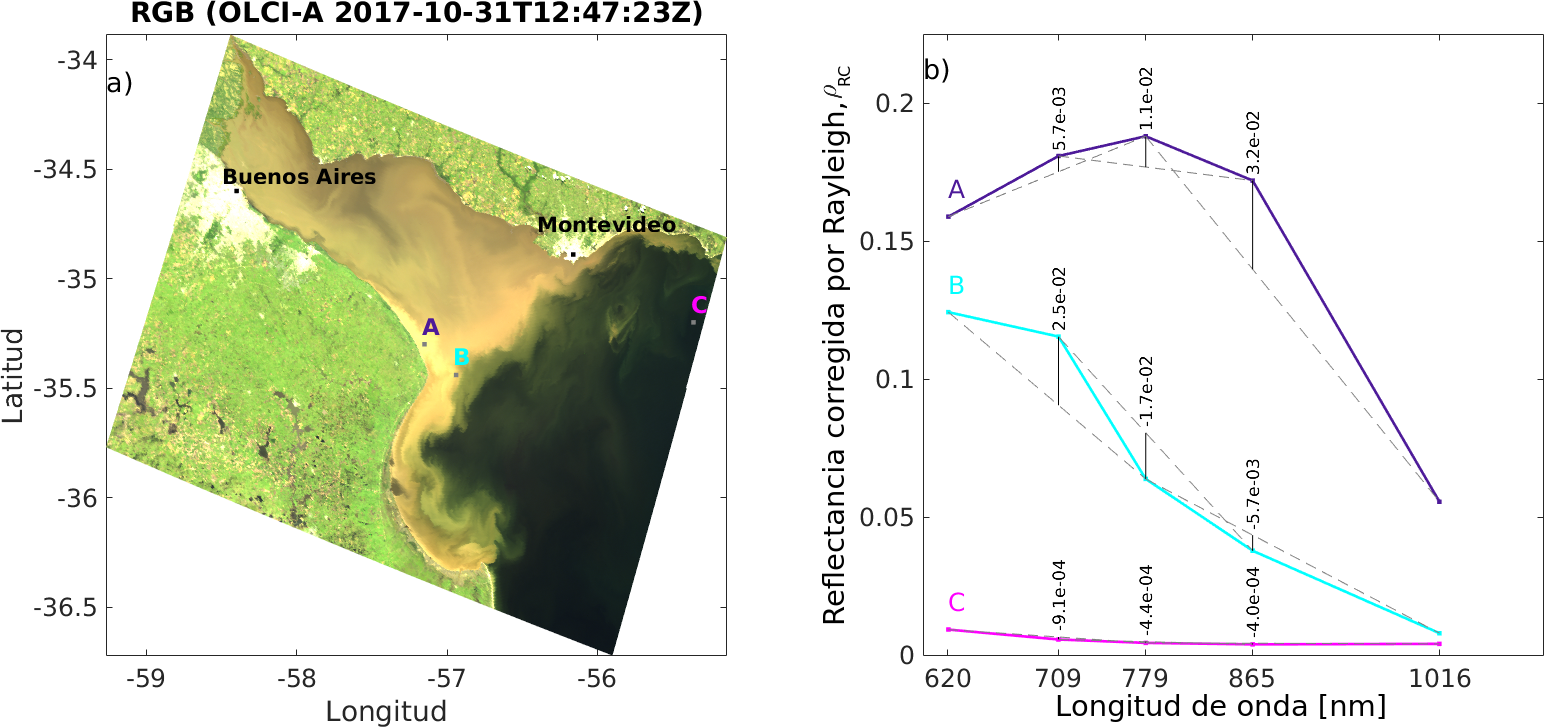
\includegraphics[width=\textwidth]{blr/figures/blrExamles}
    \caption[Ejemplos de BLRs en distintos regímenes de SPM en la imagen OLCI-A 2017-10-31T12:47:23Z sobre el RdP]{a) Composición RGB de la imagen OLCI-A en el Río de la Plata del 2017-10-31T12:47:23Z, creada a partir de reflectancias RC a 620 nm (R) 560 nm (G) y 442 nm (B). b) Reflectancias RC en las bandas roja, infrarroja cercana e infrarroja de onda corta (RNS) utilizadas para el enfoque de corrección atmosférica por BLRs (BLR-AC) en los sitios A, B y C, junto con los correspondientes valores de BLRs.}
    \label{blr:blrExamples}
    \end{figure}
    
    Otros algoritmos preexistentes en la disciplina de color del mar que usan BLRs incluyen la Altura de la Línea de Fluorescencia (\textit{Fluorescence Line Height}, FLH, \cite{letelier1996}), definida para MODIS como el BLR de las radiancias normalizadas del agua en las bandas 665 nm, 677 nm y 746 nm, es decir, $FLH = BLR(nL_{w})(665,677,746)$; el Índice de Algas Flotantes (\textit{Floating Algal Index}, FAI, Hu 2009, \cite{hu2009}), definido también para MODIS como el BLR de las reflectancias corregidas por Rayleigh a 645 nm, 859 nm y 1240 nm, es decir, $ FAI=BLR(\rho_{RC})(645,859,1240)$, el Índice de Máxima Clorofila para MERIS (Maximum Chlorophyll Index, MCI, Gower y King 2008 \cite{gower2008}, véase Ec. \ref{ppe:eq:mci}), que puede expresarse como $MCI=BLR(L_{TOA})(681,709,754)$, o el Índice Sintético de Clorofila (\textit{Synthetic Chlorophyll Index}, SCI, Shen et al. 2010, \cite{shen2010}), que se calcula utilizando reflectancias sensadas remotamente como $SCI=-BLR(R_{rs})(620,665,681)-BLR(R_{rs})(560,620,681)$ (estas bandas corresponden a los casos de MERIS y OLCI). En algunos casos, estos enfoques (FLH, SCI) se implementan después de una corrección de aerosoles, mientras que en otros casos (FAI, MCI) no se aplica.
    
    Sin embargo, todos estos enfoques son similares en el sentido que los índices BLR no se ven esencialmente afectados por señales indeseables como aerosoles y/o \textit{sunglint} moderado (y, por lo tanto, tampoco por errores típicos en el proceso de eliminación de esta señal), ya que estos componentes son generalmente espectralmente más suaves que la señal en el agua, especialmente en la región RNS. Matemáticamente, si consideramos que la señal atmosférica $\rho_{atm}$ dentro del rango espectral determinado por el triplete de bandas $(\lambda_{L},\lambda_{M},\lambda_{R})$ es lo más \textit{suave} posible, es decir, de dependencia lineal con la longitud de onda, $\rho_{atm}(\lambda)=m\lambda+b $, luego $BLR(\rho_{atm})(\lambda_{L},\lambda_{M},\lambda_{R})=0$.
    
    El algoritmo de CA presentado aquí se diseñó teniendo en cuenta que la dependencia de los BLRs con los componentes atmosféricos se minimiza mejor utilizando reflectancias RC en bandas espectralmente cercanas y para longitudes de onda más largas ($\lambda>600nm $), de forma tal de reducir el impacto de la incertidumbre proveniente de la corrección de Rayleigh, incluida la dispersión múltiple acoplada Rayleigh-aerosoles. Esto puede verse considerando la siguiente expresión para la reflectancia RC:
    
    \begin{equation}
            \rho_{RC}(\lambda) = \rho_{a}(\lambda) +  T(\lambda)\rho_{g} +  t(\lambda)\rho_{w}(\lambda)
            \label{blr:eq:rcdesc}
    \end{equation}
    
    \noindent donde asumimos que la corrección por absorción molecular (\S \ref{int:s:tAbs}) ya fue efectuada, y donde despreciamos el efecto de la espuma en superficie (\S \ref{int:s:whitecaps}).
    
    Tal como fue descrito en \S \ref{int:s:aerosoles}, las reflectancias de aerosoles pueden, en la mayoría de los casos, modelarse como funciones exponenciales de longitud de onda - similar a la Ec. \ref{int:eq:tau_aer_exp} - si se considera un rango espectral suficientemente corto en el RNS (ver Figura \ref{pca:RCvsTOA_OAA_30_OZA_30_RAA_180}, y Gordon y Wang 1994,\cite{gordon1994}, Figura 1):
    
    \begin{equation}
        \rho_{a}(\lambda_{i = L,M,R})
        \approx
        \rho_{a}(\lambda_{L})e^{-c_{\rho}\frac{\lambda_{i}-\lambda_{L}}{\lambda_{L}}}
        \label{blr:eq:aerexp} 
    \end{equation}
    
    \noindent donde generalmente $c_{\rho}$ está relacionado con el tipo de aerosol y $\rho_{a}(\lambda_{L})$ equivale a la amplitud de la exponencial en $\lambda_{L}$. Típicamente (pero no siempre) $c_{\rho}>0$, implicando una dependencia monotónica decreciente de la reflectancia con la longitud de onda.
    %
    En particular, en un rango espectral suficientemente corto, e.g. 250 nm en el RNS, es plausible aproximar la reflectancia de aerosoles como una función lineal de la longitud de onda, al menos si la comparamos con la reflectancia de aguas turbias, cuya curvatura espectral es marcadamente mayor:
    
    \begin{equation}
        \rho_{a}(\lambda_{L})e^{-c_{\rho}\frac{\lambda_{i}-\lambda_{L}}{\lambda_{L}}}
        \approx
        \rho_{a}(\lambda_{L})\left(1-c_{\rho}\frac{\lambda_{i}-\lambda_{L}}{\lambda_{L}}\right)\\
        \label{blr:eq:aerlinear}    
    \end{equation}
    
    Si la Ec \ref{blr:eq:aerlinear} se cumple para el rango espectral involucrado en el cálculo de BLR (es decir, de $\lambda_{L}$ a $\lambda_{R}$), el término de aerosoles no contribuye a $BLR(\rho_{RC})(\lambda_{L},\lambda_{M},\lambda_{R}) $, es decir: $ BLR(\rho_{a})(\lambda_{L},\lambda_{M},\lambda_{R})\approx 0$
    %
    Por otro lado, tal como fue descrito en \S \ref{int:s:sunglint}, el término de \textit{sunglint}, al menos en un régimen moderado, es esencialmente un término espectralmente blanco, especialmente en rangos espectrales cortos en la región RNS, donde podemos considerar $\frac{\partial T(\lambda)}{\partial\lambda }\approx0$, es decir, contribución insignificante a $BLR(\rho_{RC})$. Por lo tanto, considerar cualquier triplete de bandas espectralmente cercanas en el RNS implica una dependencia espectral casi lineal de los términos de la interfase atmósfera-agua en la descomposición de reflectancia RC. Por lo tanto, el $BLR(\rho_{RC})$ dependerá principalmente del término proveniente del agua:
    
    \begin{equation}
        BLR(\rho_{RC})(\lambda_{L},\lambda_{M},\lambda_{R})\approx BLR(t\rho_{w})(\lambda_{L},\lambda_{M},\lambda_{R})
        \label{blr:eq:blrrcdepw}
    \end{equation}

    \subsection{Tratamiento del Factor de Transmitancia}
    \label{blr:s:transmittance}

        Dado que la transmitancia difusa es un factor de corrección de segundo orden (\S \ref{int:s:tDif}), supondremos una expresión espectralmente blanca dentro de cada triplete considerado, cuya expresión podría depender de las condiciones geométricas y las propiedades de los aerosoles. Dicho supuesto es concomitante con la aproximación de una señal de aerosoles espectralmente lineal dentro del rango del BLR. Esta aproximación se aplica sobre la Ec. \ref{blr:eq:blrrcdepw} de la siguiente manera:
        
        \begin{equation}
            BLR(t\rho_{w})(\lambda_{L},\lambda_{M},\lambda_{R}) \approx t_{BLR}(\theta_{s},\theta_{v},\phi,a)BLR(\rho_{w})(\lambda_{L},\lambda_{M},\lambda_{R})
            \label{blr:eq:blrtfactor}
        \end{equation}
        
        \noindent donde hemos definido al factor de transmitancia equivalente como $t_{BLR}$; $\theta_{s}$, $\theta_{v}$ y $\phi$ son los ángulos de iluminación-observación (Figura \ref{int:obs_ilum}), y $a$ representa la dependencia del tipo de aerosol y su concentración. En general, al igual que cualquier factor de transmitancia, esperamos que $t_{BLR}$ sea menor que (pero cercano a) 1.
        
        Para mostrar cómo la atmósfera afecta a los BLRs calculados a partir de las bandas seleccionadas, la Figura \ref{blr:blrRcSosVsblrWAsd} muestra la relación entre $BLR(\rho_{w})$ calculada a partir de mediciones \textit{in situ}, (aplicando las Funciones de Respuesta Espectral de OLCI \cite{esasrf} y la Ec. \ref{blr:eq:blr}) y el correspondiente $BLR(\rho_{RC})$, calculado sobre reflectancias RC simuladas con el código de transferencia radiativa CNES-SOS (\S \ref{blr:s:simulations}, Cuadro \ref{blr:tab:sos}). En la Figura \ref{blr:blrRcSosVsblrWAsd}b-d, por cada $BLR(\rho_{w})$ calculado a partir de la reflectancia de agua de entrada asociada, una línea vertical (rango inter-percentil entre los percentiles 5 y 95, $IPR(5,95)$) se muestra junto con los valores extremos (representados por "$*$"), correspondientes al conjunto de reflectancias RC calculadas para la combinación de todas las condiciones atmosféricas posibles descritas en el Cuadro \ref{blr:tab:sos}. Como regla general, $BLR(\rho_{RC})$ tiende a presentar valores absolutos más bajos que $BLR(\rho_{w})$ - es decir que para valores negativos $BLR(\rho_{RC})$ es mayor que $BLR(\rho_{w})$ y para valores positivos es menor - como lo sugieren las pendientes de las regresiones lineales (i.e. $m<1$). En términos de forma espectral, los BLRs absolutos más bajos están asociados a señales espectralmente más suaves, lo que es consistente con un factor de transmitancia equivalente menor que 1 (ver Ecs. \ref{blr:eq:blrrcdepw} y \ref{blr:eq:blrtfactor}). Todos los escenarios asociados a los valores mínimos/máximos, representados por "$*$", corresponden a casos en los que el sensor se coloca en ángulos recíprocos del sol ($\theta_{s}=\theta_{v}$ y $\phi=180\degree$, es decir, \textit{sunglint} directo). Además de estos casos excepcionales, los bajos sesgos obtenidos de las regresiones lineales ($b$) son consistentes con los supuestos subyacentes a la Ec. \ref{blr:eq:blrrcdepw}, es decir, $BLR(\rho_{a}+T\rho_{g})\approx0$.
        
        \begin{figure}
        \centering
        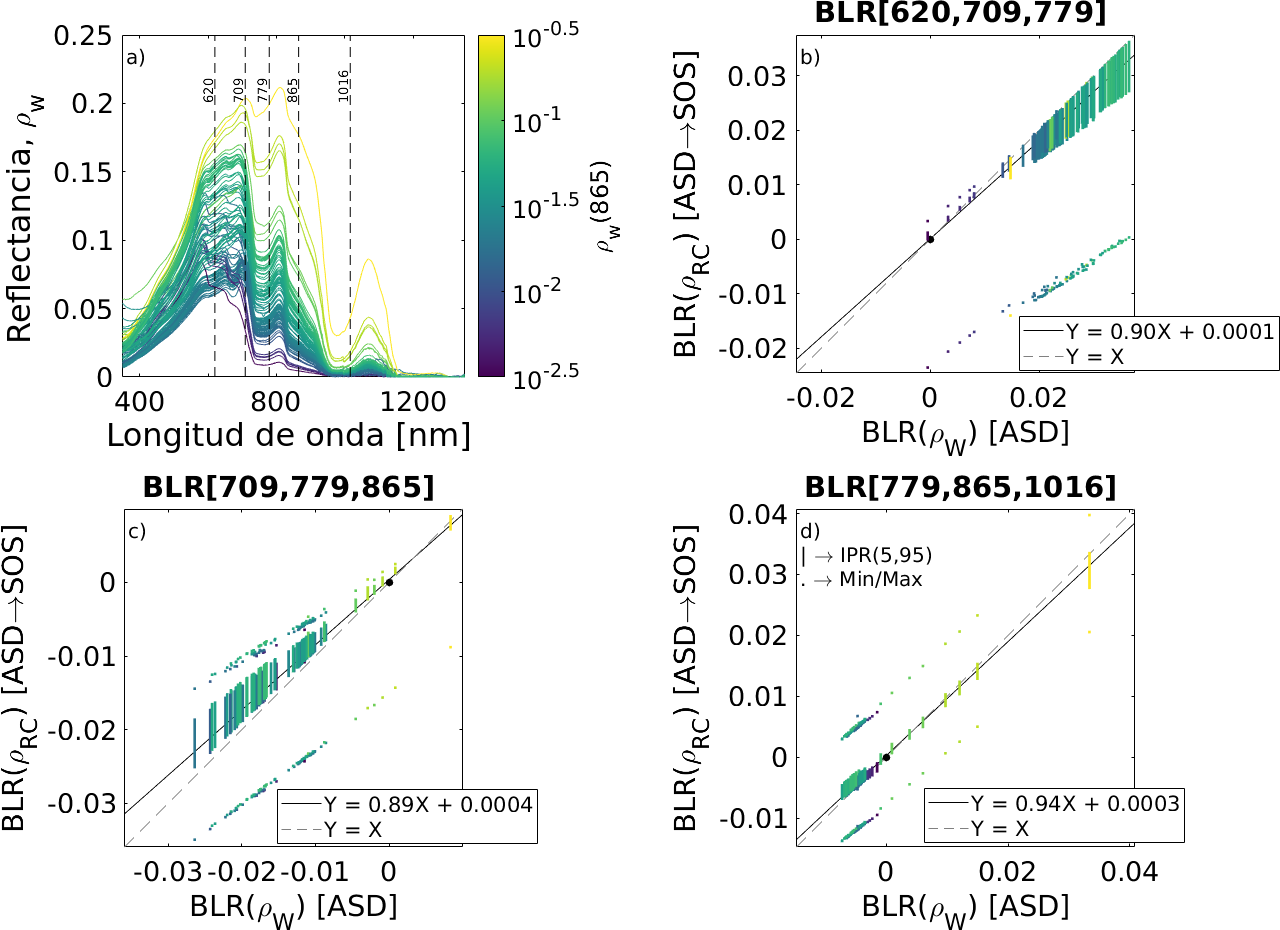
\includegraphics[width=\textwidth]{blr/figures/blrRcSosVsblrWAsd}
        \caption[Comparación entre BLRs de reflectancias del agua medidas y de reflectancias RC simuladas]{a) Reflectancias hiperespectrales obtenidas mediante mediciones radiométricas \textit{in situ} (\S \ref{blr:s:insitu}), utilizadas como reflectancias del agua de entrada en el código de transferencia radiativa CNES-SOS (\S \ref{blr:s:simulations}). Relación entre $BLR(\rho_{w})$ (de las mediciones \textit{in situ}) y $BLR(\rho_{RC})$ (de mediciones \textit{in situ} y simulaciones) para los tripletes $(620,709,779)$ (b), $(709,779,865)$ (c) y $(779,865,1016)$ (d).}
        \label{blr:blrRcSosVsblrWAsd}
        \end{figure}
        
        En todo el conjunto de simulaciones se observó que la dependencia de $t_{BLR}$ con las condiciones geométricas podría reducirse a una sola variable, el factor geométrico de masa de aire, $\mu$ (Ec. \ref{int:eq:mu}) ya que, a excepción de los escenarios con \textit{sunglint} directo, se observó que el acimut relativo tiene un efecto muy pequeño en $t_{BLR}$. Este hecho está bien ilustrado en la Figura \ref{blr:tramsittance}, donde $t_{BLR}$ y su sesgo se representan frente al factor de masa de aire considerando la siguiente expresión:
        
        \begin{equation}
            BLR(\rho_{RC}) = t_{BLR}(\mu)BLR(\rho_{w}) + sesgo(\mu)
            \label{blr:eq:blrtmufactor}
        \end{equation}
        
        En la Figura \ref{blr:tramsittance}, cada punto representa el resultado de $t_{BLR}$ (recuadros superiores) y su correspondiente sesgo (recuadros inferiores) al haber aplicado una regresión lineal de la forma de la Ec. \ref{blr:eq:blrtmufactor} realizada sobre los diferentes subconjuntos definidos por valores específicos para $\theta_{s}$, $\theta_{v}$ y $\phi$, es decir, para condiciones geométricas específicas. Se puede observar que: i) los sesgos son usualmente menores a $0.001$, por lo que no serán tenidos en cuenta en la corrección general de transmitancia, y ii) la dependencia de $t_{BLR}$ con $\mu$ puede considerarse lineal en el rango $\mu\in[2;4]$. Se observan resultados similares al aumentar los espesores ópticos de aerosoles.

        \begin{figure}
        \centering
        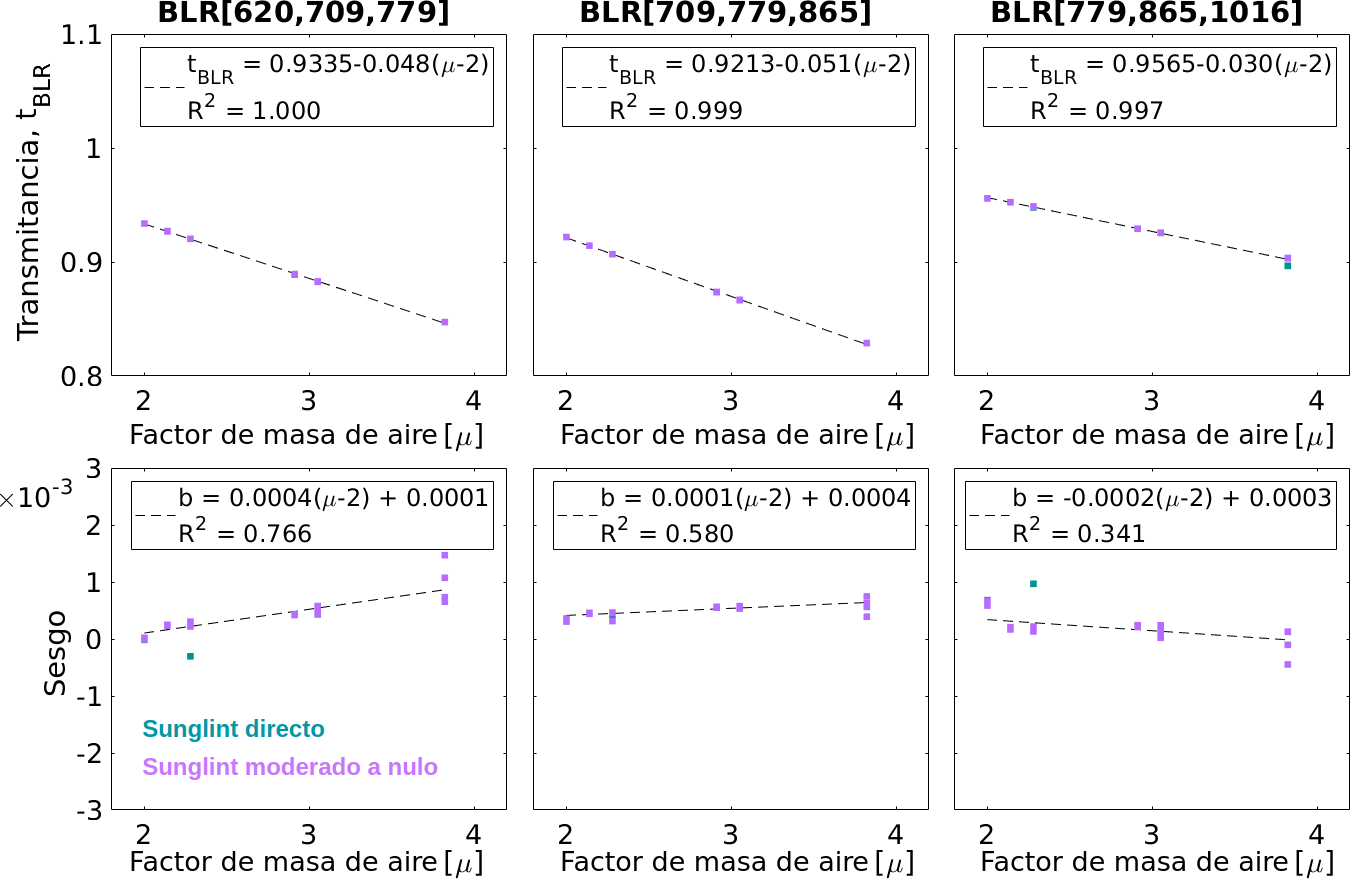
\includegraphics[width=\textwidth]{blr/figures/teqVsMu}
        \caption[Transmitancias equivalentes ($t_{BLR}$) y sesgos vs. factor geométrico de masa de aire para cada BLR utilizado en el esquema BLR-AC.]{Transmitancias equivalentes ($t_{BLR}$, Ecs. \ref{blr:eq:blrtfactor} y \ref{blr:eq:blrtmufactor}) y sesgos vs. factor geométrico de masa de aire, $\mu = \frac{1}{cos(\theta_{s})} + \frac{1}{cos(\theta_{v})}$, para cada BLR utilizado en este trabajo. Los puntos turquesa (violeta) representan los resultados sobre subconjuntos correspondientes a diferentes geometrías de observación/iluminación con (sin) la presencia de \textit{sunglint} directo. Las líneas punteadas indican las regresiones lineales.}
        \label{blr:tramsittance}
        \end{figure}
        
        Sobre la base de estos resultados, los BLRs calculados sobre de escenas RC OLCI utilizadas para estimar la señal del agua son divididos por los factores de transmitancia equivalentes correspondientes para cada píxel (Figura \ref{blr:tramsittance}), para así poder estimar los BLRs asociados a la señal de agua en escenas OLCI, es decir:

        \begin{equation}
            BLR(\rho_{w,OLCI}) := \frac{BLR(\rho_{RC,OLCI})}{t_{BLR}(\mu)}
            \label{blr:eq:blrtolcifactor}
        \end{equation}
        
    \subsection{Relación entre los BLRs y las reflectancias del agua}
    \label{blr:s:blrrhow}

        Las secciones anteriores de este capítulo describieron por qué $BLR(\rho_{w})(620,709,779)$, $BLR(\rho_{w})(709,779,865)$ y $BLR(\rho_{w})(779,865,1016)$ (Ecs. \ref{blr:eq:blr}, \ref{blr:eq:blrrcdepw} y \ref{blr:eq:blrtfactor}) representan un conjunto conveniente de cantidades para estimar la reflectancia del agua en cualesquiera de las bandas consideradas. En este capítulo, nos centramos en establecer una relación entre los BLRs y las reflectancias del agua en al menos dos bandas: 865 nm y 1016 nm, ya que este es el mínimo requerido para eventualmente extrapolar la señal atmosférica a longitudes de onda más cortas (mediante un procedimiento de extrapolación similar al descrito en Gordon y Wang 1994, \cite{gordon1994}).
        Decidimos usar un subconjunto de imágenes OLCI para lograr un conjunto de calibración plausible, a fin de evitar errores sistemáticos que pudieren inducirse al calibrar el algoritmo con datos provenientes de otras fuentes (como mediciones \textit{in situ} o simulaciones de transferencia radiativa).
        Para construir este conjunto de datos, se seleccionó un total de 13 subregiones de 9 imágenes del RdP libres de nubes, \textit{sunglint} o neblina (ver Cuadro \ref{blr:tab:olci}, recuadros magenta en la Figura \ref{blr:Blr14CalValDataSet}). Sobre estas subregiones, se aplicó una CA no operativa para inferir la reflectancia del agua en las bandas de 865 nm y 1016 nm, basándonos en la estimación del componente atmosférico a partir de ventanas de agua clara seleccionadas manualmente - cercanas a las ventanas de interés - de $15 \times 15$ píxeles. Dicha corrección no operativa es denominada en este documento \textit{Fix-AC} (consulte el Cuadro \ref{blr:tab:olci}, recuadros blancos en la Figura \ref{blr:Blr14CalValDataSet}) y supone, para la imagen considerada, un tipo y concentración de aerosoles horizontalmente homogéneos.
        
        \begin{figure}
        \centering
        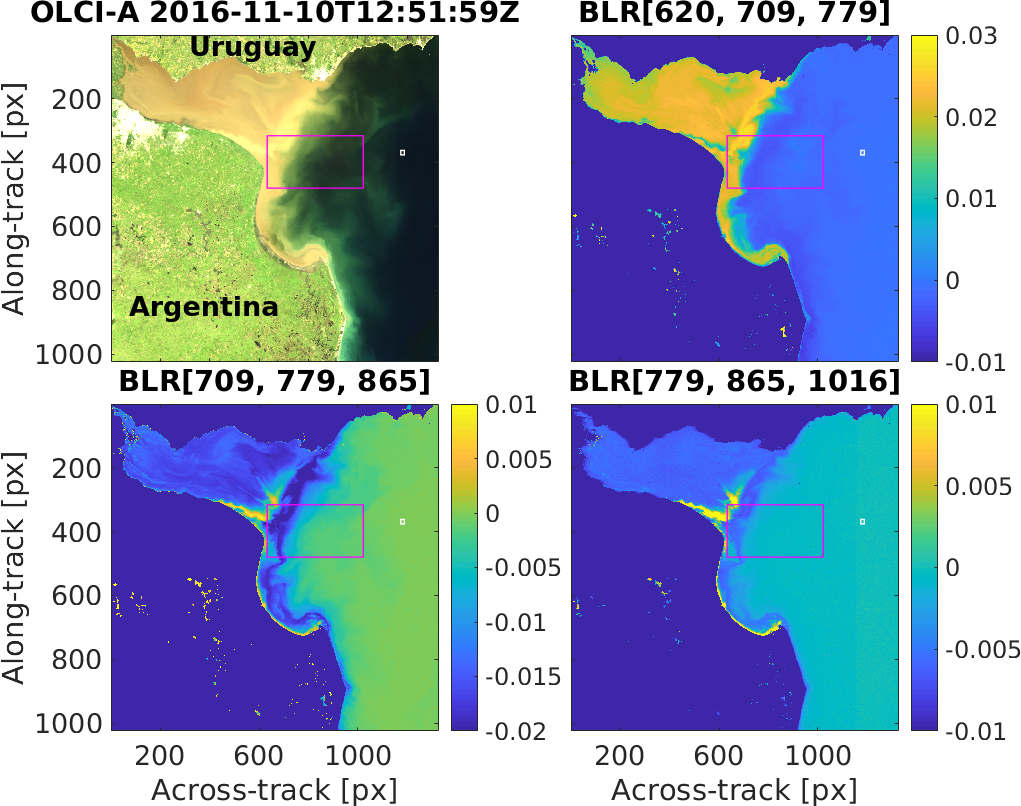
\includegraphics[width=0.8\textwidth]{blr/figures/Blr14CalValDataSet}
        \caption[Ejemplo de una escena que forma parte del conjunto de datos utilizado para calibrar la relación $BLR(\rho_{w})$ vs. $\rho_{w}$.]{Ejemplo de una escena que forma parte del conjunto de datos utilizado para calibrar la relación $BLR(\rho_{w})$ vs. $\rho_{w}$. El cuadro magenta encierra el subconjunto seleccionado de la imagen agregada al conjunto de datos de calibración, mientras que la señal de aerosoles se sustrajo usando el esquema de corrección atmosférica de Ventana Clara Fija (Fix Clear Window, Fix-AC, Ec. \ref{blr:eq:rhow}) de $15 px \times 15 px$, indicadas por los recuadros blancos.}
        \label{blr:Blr14CalValDataSet}
        \end{figure}
        
        Estas \textit{ventanas claras} se eligieron para estar lo más cerca posible de la subregión de interés y a su vez estar totalmente libres de señal de agua en el RNS (determinado por inspección visual de los rásteres $\rho_{RC}$). Esta simple eliminación de aerosol supone una señal atmosférica espacialmente uniforme que se resta de toda la subregión de interés de la siguiente manera:
        
        \begin{equation}
            \rho_{w} = \frac{\rho_{RC} - \rho_{a}^{VentClara}}{t(\lambda)}
            \label{blr:eq:rhow}
        \end{equation}
        
        \noindent donde utilizaremos la expresión simple para el factor de transmitancia difusa dada en la Ec. \ref{int:eq:tDif}, pero en ausencia de aerosoles, $\tau_{a}=0$. Una vez realizado este proceso, el conjunto de datos de calibración formado por las subregiones mencionadas se usa para ajustar una superficie de calibración en el subespacio tridimensional BLR, que es generado por $BLR(620,709,779)$, $BLR(709,779,865)$ y $BLR(779,865,1016)$ (Figuras \ref{blr:Blr14CalValDataSet} y \ref{blr:blr3d}). La superficie de calibración se genera mediante una cuadrícula de malla bidimensional de $X$ - es decir, $BLR(620,709,779)$ - en el rango $(-0.0100;0.0350)$ (paso $0.0005$) e $Y$ - es decir, $BLR(709,779,865)$ - en el rango $(-0.0300;0.0150)$ (paso $0.0005$). Los valores de $Z$ - $BLR(779,865,1016)$ - en cada punto de la cuadrícula se toman como la mediana de los valores $Z$ tomados por el conjunto de datos de calibración en el par $(X,Y)$ correspondiente. Esto se puede hacer de esta manera ya que la superficie BLR no presenta ambigüedad en $Z$, es decir, la superficie BLR puede considerarse como una función de $(X,Y)$: $Z=f(X,Y)$. El punto de calibración se descarta si menos de 10 datos satelitales caen dentro del rango $(X,Y)$ asociado.
        %
        El triplete $BLR(\rho_{w})$ asignado a cada píxel de entrada será el triplete $BLR(\rho_{w})$ más cercano (en el sentido euclidiano) correspondiente a la curva de calibración, junto con la reflectancia del agua en 865 nm y 1016 nm.
        
        \begin{figure}
        \centering
        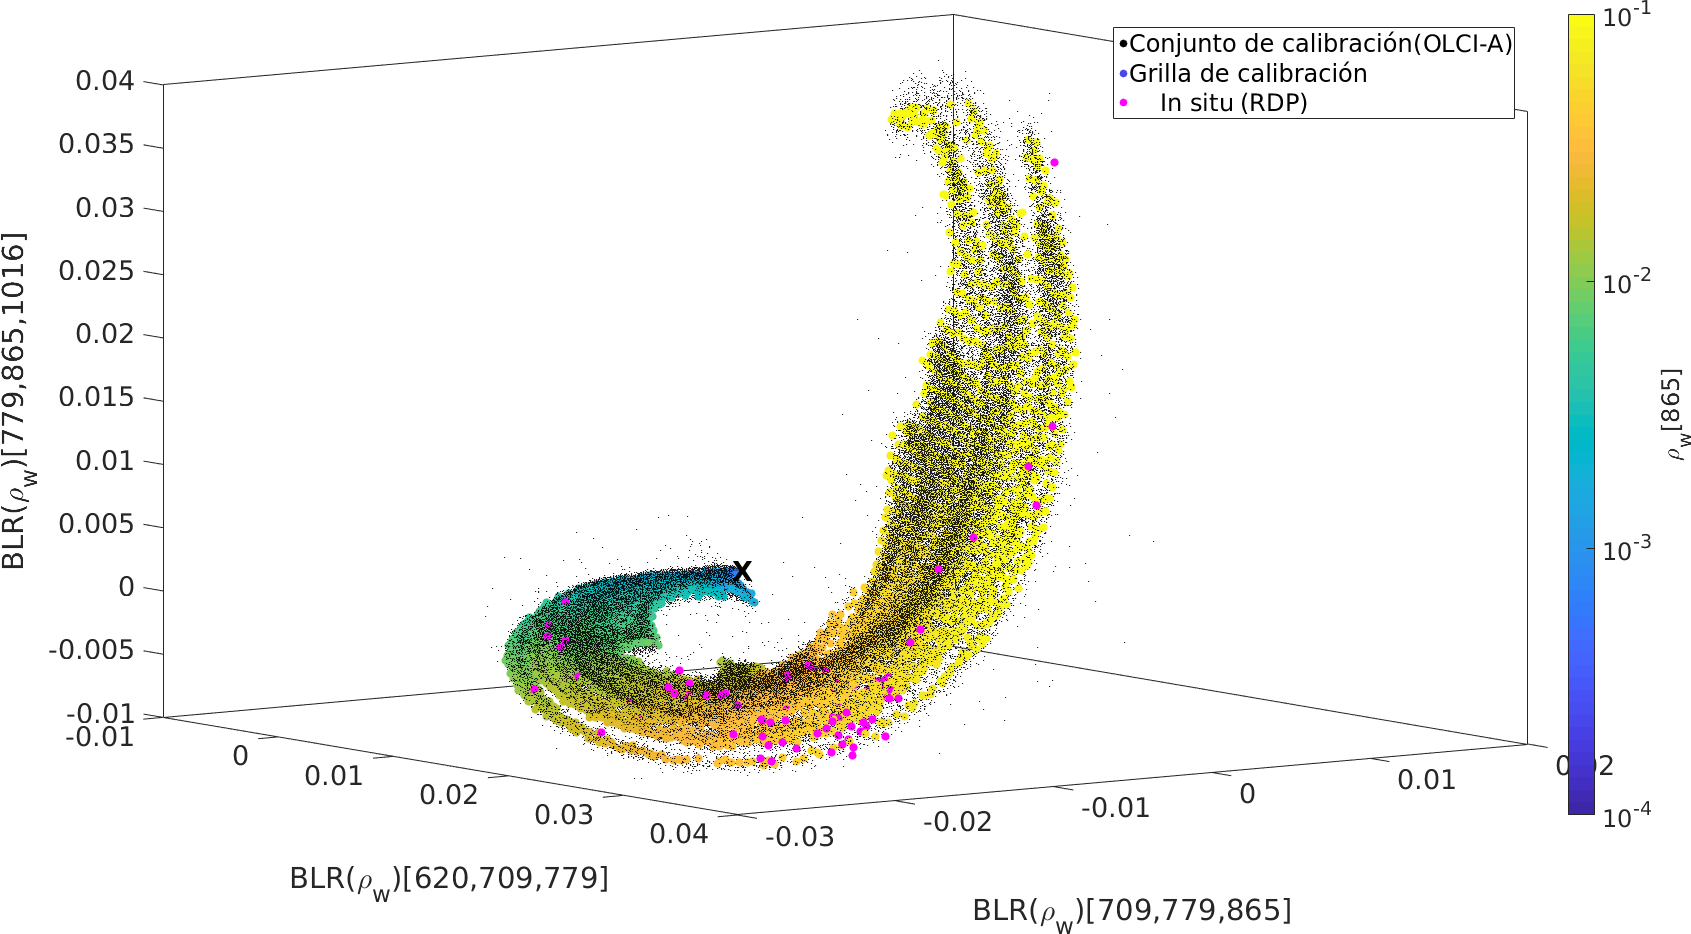
\includegraphics[width=\textwidth]{blr/figures/blr3D}
        \caption[Espacio tridimensional $BLR(\rho_{w})$, formado por los tres BLR linealmente independientes definidos por los tres tripletes consecutivos de las cinco bandas OLCI en 620, 709, 779, 865 y 1016 nm.]{Espacio tridimensional $BLR(\rho_{w})$, formado por los tres BLR linealmente independientes definidos por los tres tripletes consecutivos de las cinco bandas OLCI en 620, 709, 779, 865 y 1016 nm. Puntos pequeños: conjunto de datos de calibración OLCI-A. Puntos grandes mapeados en color: superficie de calibración obtenida del conjunto de datos de calibración OLCI-A, cuyo color indica reflectancia del agua a 865 nm. Los puntos magentas son datos \textit{in situ}. El origen se indica con una X y corresponde a un escenario de \textit{aguas claras}, Ec. \ref{int:eq:blackPixelAmplitud}.}
        \label{blr:blr3d}
        \end{figure}

    \subsection{Elección de bandas}
    \label{blr:s:bandchoice}
    
        En este capítulo, hemos optado por utilizar las reflectancias RC calculadas a partir de las bandas OLCI en 620, 709, 779, 865 y 1016 nm. Estas 5 bandas conforman un espacio $\mathbb{R}^{5}$, del cual consideramos un subespacio conformado por tres BLRs consecutivos, linealmente independientes: $BLR(\rho_{RC})(620, 709, 779)$, $BLR(\rho_{RC})(709, 779, 865)$ y $BLR(\rho_{RC})(779, 865, 1016)$. Estas bandas se han elegido para i) maximizar el impacto de la señal del agua (turbia) en $BLR(\rho_{RC})$, y simultáneamente ii) minimizar el impacto de los componentes atmosféricos. No se consideraron otras bandas OLCI dentro de esta región espectral, por ej. aquellas en el rango de 760-770 nm y la banda centrada a 940 nm, ya que están fuertemente afectadas por la absorción de gases troposféricos (\S \ref{int:s:tAbs}). Las bandas OLCI en el rango de 660-690 nm también se evitan porque las reflectancias del agua pueden verse afectadas por la absorción y la fluorescencia de la clorofila (véase Figura \ref{dat:HyperTriOS}).

    \subsection{Estimación de la reflectancia de aerosoles en las bandas 865 nm y 1016 nm}
    \label{blr:s:residual}

        La reflectancia de aerosoles, $\rho_{a}$, en 865 nm y 1016 nm es computada para testear el grado de correlación espacial con la reflectancia del agua estimada - que se espera sea baja - utilizando la siguiente expresión simplificada:
        
        \begin{equation}
            \rho_{a}(\lambda) = \rho_{RC}(\lambda) - t(\lambda,\mu)\rho_{w,j}(\lambda)
            \label{blr:eq:residual}
        \end{equation}
        
        \noindent donde $\rho_{w,j}$ es el valor de reflectancia del agua asignado al vecino euclidiano más cercano desde la superficie de calibración en el espacio BLR.
        El factor de transmitancia difusa se calculó también utilizando la Ec. \ref{int:eq:tDif} a $\tau_{a}=0$. Esta misma expresión se aplicó para intercomparar con las reflectancias en aerosol producidas por otros esquemas preexistentes (BAC/BPAC y SeaDAS-2(865,1016)).
        Se realiza una última corrección en $\rho_{a}(865)$ para restringir el valor se $\epsilon_{a}(865,1016)=\frac{\rho_{a}(865)}{\rho_{a}(1016)}$ dentro del rango de $(0.85; 1.25)$. Estos límites se determinaron como los valores extremos tomados en un conjunto de 82 ventanas diferentes de tamaño $15px \times 15px$ de escenas OLCI-A de regiones de aguas claras cerca del Río de la Plata, Bahía Blanca, Mar del Norte, Mar Amarillo, Amazonas y el norte de Australia. Además, estos límites son consistentes con lo que se obtuvo sobre las simulaciones CNES-SOS. Esta corrección se realiza imponiendo la siguiente condición píxel a píxel:
        
        \begin{equation}
            0.85\rho_{a}(1016) \leq \rho_{a,new}(865) \leq 1.25\rho_{a}(1016)
            \label{blr:eq:epsCorr}
        \end{equation}

        y luego, corrigiendo consecuentemente los valores de $\rho_{w}(865)$ obtenidos. Esta restricción asume como más confiables los valores estimados de $\rho_{w}(1016)$ por sobre los de $\rho_{w}(865)$ cuando el $\epsilon_{a}(865,1016)$ estimado cae fuera del rango esperado de variabilidad natural y se discute más en la \S \ref{blr:s:discussion}.

    \subsection{Esquema de corrección atmosférica: resumen}
    \label{blr:s:summary}

    La siguiente enumeración resume el algoritmo de CA desarrollado en el presente capítulo:
    
    \begin{enumerate}
        \item La corrección por EPVs (\S \ref{ppe}) se aplica en las imágenes L1B (radiancias a TOA).
        \item La corrección por Rayleigh (y absorción gaseosa) se aplica utilizando el software SeaDAS v7.5.
        \item Se calculan $BLR(\rho_{RC})(620,709,779)$, $BLR(\rho_{RC})(709,779,865)$ y $BLR(\rho_{RC})(779,$ $865,1016)$ a partir de las correspondientes reflectancias corregidas por Rayleigh (ver \S \ref{blr:s:atb} - \ref{blr:s:bandchoice}, Ec. \ref{blr:eq:blr}).
        \item Se aplica una corrección del factor de transmitancia para relacionar $BLR(\rho_{RC})$ con $BLR(\rho_{w})$ (véase \S \ref{blr:s:transmittance}, Ec. \ref{blr:eq:blrtolcifactor})
        \item Para cada píxel, los BLRs calculados se asocian al triplete de BLRs desde la superficie de calibración que minimizan la distancia euclidiana en el espacio BLR. Se asigna al píxel en cuestión la reflectancia del agua correspondiente a 865 nm y 1016 nm (\S \ref{blr:s:blrrhow}).
        \item La señal atmosférica en estas bandas se obtiene restando la señal de agua asignada (habiéndole aplicado un factor de transmitancia difusa) a la reflectancia RC (\S \ref{blr:s:residual}, Ec. \ref{blr:eq:residual}).
        \item Se aplica una restricción final a $\rho_{a}(865)$ para limitar $\epsilon_{a}(865,1016)$ dentro del rango razonable de $(0.85; 1.25)$ (\S \ref{blr:s:residual}, Ec. \ref{blr:eq:epsCorr}).
    \end{enumerate}
    
    % \begin{figure}
    % \centering
    % 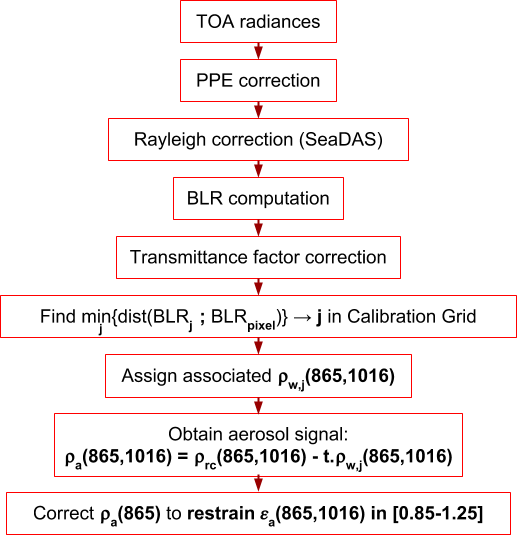
\includegraphics[width=7 cm]{blr/figures/blrScheme}
    % \caption{Esquema de corrección atmosférica por BLR (BLR-AC), detallado en el resumen.}
    % \label{blr:scheme}
    % \end{figure}
    
    Este abordaje puede extenderse a todo el rango de bandas de interés restando la reflectancia del agua estimada en el NIR a la reflectancia a TOA (con la adecuada aplicación del factor de transmitancia difusa) y aplicando la suposición de píxeles claros para extrapolar la señal de aerosoles a longitudes de onda más cortas (Gordon y Wang 1994, \cite{gordon1994}, Stumpf et al. 2003, \cite{stumpf2003}).
    
    \subsection{Efecto del ruido del sensor sobre los BLRs}
    \label{blr:s:blrNoise}

        \subsubsection{Cómputo del ruido absoluto del sensor}
        \label{blr:s:blrNoiseHA}
            Para analizar el alcance del ruido sobre las bandas OLCI involucradas en el cómputo de los BLRs, se estimó el error asociado al ruido del sensor para todas las bandas utilizadas. Para ello, se utilizaron 82 ventanas de $15 px \times 15 px$ de imágenes L2 de reflectancias corregidas por Rayleigh (habiendo utilizado SeaDAS al igual que en \S \ref{blr:s:olci}) cercanas al RdP en condiciones de cielo despejado y aguas claras, lo cual equivaldría en el RNS a condiciones de baja variabilidad espacial dentro de las ventanas. De esta forma, es posible aplicar el método de \textit{Área Homogénea} propuesto por Duggin et al. 1985, \cite{duggin1985}. Dicho método consiste en asociar el desvío estándar sobre dichas ventanas al ruido en la imagen, de forma tal de que
            
            \begin{equation}
                \sigma(\rho_{RC}(\lambda_{i})) = \frac{1}{N}\sum_{j=1}^{N} \sigma(\rho_{RC}^{j}(\lambda_{i}))
                \label{blr:eq:noiseHA}
            \end{equation}
            
            \noindent
            corresponda al valor absoluto del ruido sobre la reflectancia RC estimado para la banda centrada en $\lambda_{i}$ (aquí $\sigma(\cdot)$ representa el desvío estándar). En esta ecuación, $\rho_{RC}^{j}(\lambda_{i})$ es el ráster de la reflectancia RC de la banda $\lambda_{i}$ para la $j$-ésima ventana de 
            $15 px \times 15 px$ considerada, $N$ es el número de imágenes consideradas y $std(\cdot)$ es el desvío estándar.
            
            A partir de este análisis se obtuvieron los valores de ruido absoluto reportados en el Cuadro \ref{blr:tab:blrNoise} para las bandas 620, 709, 779, 865 y 1016 nm. Dichos valores fueron luego utilizados para estimar la propagación del ruido del sensor sobre los BLRs.
            %
            En este procedimiento utilizaremos el ruido absoluto y no la relación señal-ruido (SNR) dado que esta última siempre es referida a un valor de radiancia/reflectancia típico, valor que \textit{a priori} se desconoce o bien está referido a aguas claras.
            
            \begin{table}
            \caption{Valores absolutos del ruido sobre las reflectancia RC de las bandas 620, 709, 779, 865 y 1016 nm de OLCI-A obtenidos mediante el método de \textit{Área Homogénea}.}
            \begin{tabular}{|l|l|l|l|l|l|}
            \hline
            \textbf{Banda}, $[nm]$            & \textbf{620} & \textbf{709} & \textbf{779} & \textbf{865} & \textbf{1016} \\ \hline
            \textbf{Ruido}, $\sigma[10^{-4}]$ & 5.610        & 4.868        & 4.925        &  4.812       &  8.059        \\ \hline
            \end{tabular}
            \label{blr:tab:blrNoise}
            \end{table}

        \subsubsection{Propagación del ruido del sensor sobre los BLRs}
        \label{blr:s:blrNoiseBLR}
            
            Tal como lo expuesto por Curran et al. 1989, \cite{curran1989}, o por Gross et al. 2007, \cite{gross2007}, podremos asumir que el ruido del sensor es independiente de la señal natural y lo consideramos como una variable aleatoria normal aditiva, es decir:
            
            \begin{equation}
                \rho_{RC}(\lambda_{i}) \rightarrow \rho_{RC}(\lambda_{i}) + \varepsilon(\lambda_{i}) =  \rho_{RC}(\lambda_{i}) + \mathcal{N}(0,\sigma_{i})
                \label{blr:eq:rhoRCNoise}
            \end{equation}

            \noindent siendo $\mathcal{N}(0,\sigma_{i})$ una variable aleatoria de distribución normal de media $0$ y desvío estándar $\sigma_{i}$. Para entender cómo se propaga el ruido del sensor en el cálculo de los BLRs, observemos que las Ecs. \ref{blr:eq:blr} y \ref{blr:eq:baseline} pueden ser rescritas como combinación lineal de las reflectancias dentro del triplete considerado:
            
            \begin{equation}
                BLR(\rho_{RC})[\lambda_{L},\lambda_{M},\lambda_{R}] = \sum_{i=L,M,R} A_{i}\rho_{RC}(\lambda_{i}) \rightarrow \sum_{i=L,M,R} A_{i}\rho_{RC}(\lambda_{i}) + \varepsilon(\lambda_{i})
                \label{blr:eq:blrCL}
            \end{equation}

            \noindent
            donde las $A_{i}$ son constantes que dependen únicamente de las longitudes de onda de las bandas de cada triplete y se reportan en el Cuadro \ref{blr:tab:blrCoef}.

            \begin{table}
            \caption{Coeficientes que acompañan a las reflectancias RC en el cálculo de los BLRs (Ec. \ref{blr:eq:blrCL}).}
            \begin{tabular}{|l|l|l|l|}
            \hline
            \textbf{Bandas/Coeficientes}    & \textbf{$A_{L}$} & \textbf{$A_{M}$} & \textbf{$A_{R}$} \\ \hline
            \textbf{$BLR(\rho)[620,709,779] $} & -0.440252               & 1                       & -0.559748               \\ \hline
            \textbf{$BLR(\rho)[709,779,865] $} & -0.551282               & 1                       & -0.448718               \\ \hline
            \textbf{$BLR(\rho)[779,865,1016]$} & -0.637131               & 1                       & -0.362869               \\ \hline
            \end{tabular}
            \label{blr:tab:blrCoef}
            \end{table}

            \noindent
            entonces es válido considerar que cada BLR será a su vez una variable aleatoria de distribución normal cuyo desvío estándar se expresa de la siguiente manera.

            \begin{equation}
                \sigma_{BLR}^{2} = \sum_{i=L,M,R}A_{i}^{2}\sigma_{i}^{2}
                \label{blr:eq:blrNoiseCL}
            \end{equation}
            
            Considerando esta expresión y el hecho de que los valores de $A_{i}$ son menores a la unidad para las bandas laterales ($i=L$ e $i=R$), se desprende que el aporte del ruido del sensor en las bandas laterales será comparativamente menor al de la banda central ($i=M$). Por ejemplo, dado que $A_{1016} = -0.362869$ en el cálculo de $BLR(\rho_{RC})[779,865,1016]$, el aporte del ruido de la banda de 1016 nm a este BLR - la banda con ruido más elevado dentro del conjunto considerado - será de $\approx 13 \%$ del ruido original de dicha banda.

%%%%%%%%%%%%%%%%%%%%%%%%%%%%%%%%%%%%%%%%%%
\section{Resultados}
\label{blr:s:results}

    \subsection{BLRs en aguas claras y turbias}
    \label{blr:s:results:blrs}

        El hecho de que los BLRs considerados en la región espectral RNS se acercan a valores cercanos a cero en aguas claras es consistente con lo expresado en la Ec. \ref{blr:eq:blrrcdepw}, suponiendo que las aguas muy claras son en realidad negras en el RNS para un sensor remoto óptico. Esta propiedad se ve claramente a partir de las reflectancias RC de OLCI, y es evidente en la Figura \ref{blr:blrHist} (así como en las Figuras \ref{blr:blrExamples} y \ref{blr:Blr14CalValDataSet}), donde se intercomparan las distribuciones de BLRs provenientes de i) ventanas seleccionadas para realizar la calibración BLR-AC (que contienen principalmente aguas turbias, \textit{ventanas de calibración} en el Cuadro \ref{blr:tab:olci}), y ii) ventanas seleccionadas para realizar el esquema Fix-AC (que contienen aguas muy claras, \textit{ventanas Fix-AC} en el Cuadro \ref{blr:tab:olci}). En la Figura \ref{blr:blrHist} se observa que los valores medios de BLR y los rangos intercuartiles (IQR) sobre las ventanas Fix-AC se aproximan a 0 (siempre menores que $10^{-3}$) y que los IQRs estimados en dichas ventanas son al menos 9 veces más pequeños que los IQRs calculados para las ventanas de calibración.
        Esto es consistente con lo que se ha predicho y muestra que para este enfoque, el supuesto de agua negra se traduce a la condición $BLR(\rho_{w})=0$ (también evidente al observar las regiones de agua clara en la Figura \ref{blr:Blr14CalValDataSet}). Esto significa que, dado un píxel donde simultáneamente $BLR(\rho_{w})=0$ para los tres tripletes considerados, el algoritmo estima $\rho_{w}(865)=\rho_{w}(1016)=0 $, es decir, el algoritmo vuelve naturalmente al enfoque estándar de CA para aguas claras.
        
        \begin{figure}
        \centering
        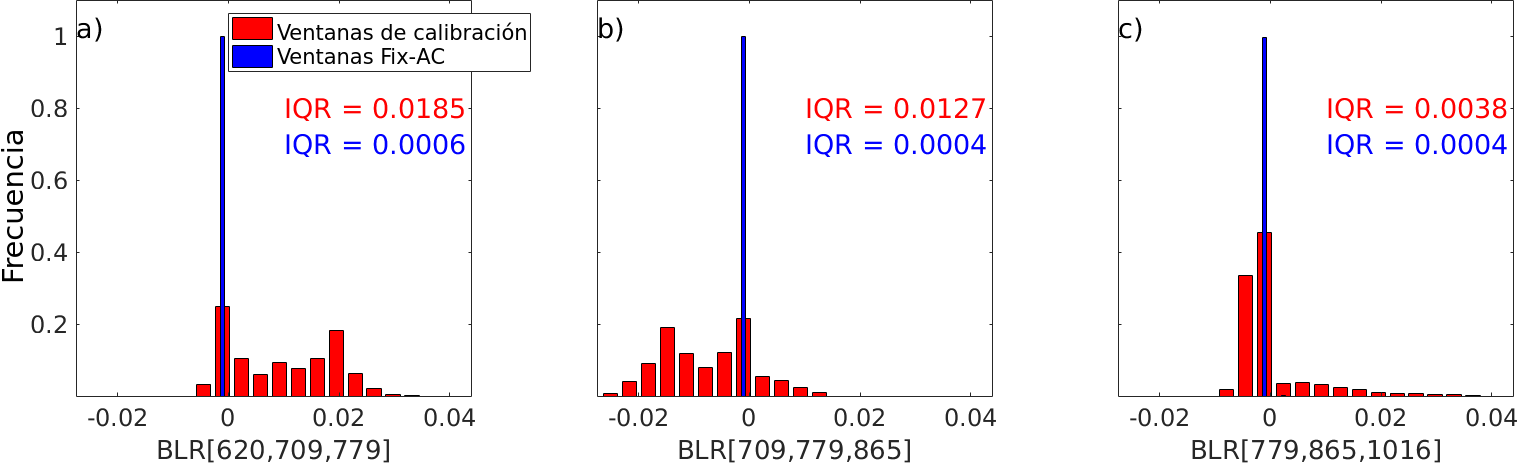
\includegraphics[width=\textwidth]{blr/figures/blrHistClearVsTurbid}
        \caption[Histogramas de $BLR(\rho_{w})$ en los tripletes $(620,709,779)$ nm (a), $(709,779,865)$ nm (b) y $(779,865,1016)$ nm (c) para el conjunto completo de ventanas de calibración y para las ventanas de aguas claras.]{Histogramas de $BLR(\rho_{w})$ en los tripletes $(620,709,779)$ nm (a), $(709,779,865)$ nm (b) y $(779,865,1016)$ nm (c) para: el conjunto completo de ventanas de calibración (en rojo, Cuadro \ref{blr:tab:olci}) y para las ventanas de aguas claras (en azul, ventanas Fix-AC en el Cuadro \ref{blr:tab:olci}), mostrando que los BLRs se aproximan a 0 en aguas claras.}
        \label{blr:blrHist}
        \end{figure}
        
        Esto también es evidente en la Figura \ref{blr:blrVsRho}, donde se intercompara la relación $BLR$ vs. $\rho_{w}$ proveniente de tres fuentes diferentes de información para mostrar cómo los BLRs en cada uno de los tres tripletes de longitudes de onda considerados varían según las reflectancias del agua a 865 nm y 1016 nm. Los puntos azules muestran datos de las ventanas de calibración (Cuadro \ref{blr:tab:olci}); en magenta, los BLRs calculados a partir de los datos \textit{in situ} recopilados del Río de la Plata (\S \ref{blr:s:insitu}), y una familia de curvas de colores muestran la relación $BLR$ vs. $\rho_{w}$ usando un modelo de reflectancia basado en la Aproximación de Dispersión cuasi-Simple (quasi-Single Scattering Albedo, qSSA), descrito en \S \ref{qssa}. Esta familia de curvas fue construida asumiendo que en las bandas del RNS consideradas la única componente bioóptica influyente en aguas turbias del RdP es el material particulado en suspensión. Para estas curvas se fijaron los coeficientes de dispersión y absorción específicos de partículas (descritos en \S \ref{qssa:s:iops_spm}), a excepción del parámetro de absorción de partículas a 443 nm que se varió en el rango $[0.021-0.062]g/m^{2}$ y donde el material particulado en suspensión (SPM) varió logarítmicamente entre $0.001 g/m^{3}$ y $10000 g/m^{3}$.

        \begin{figure}
        \centering
        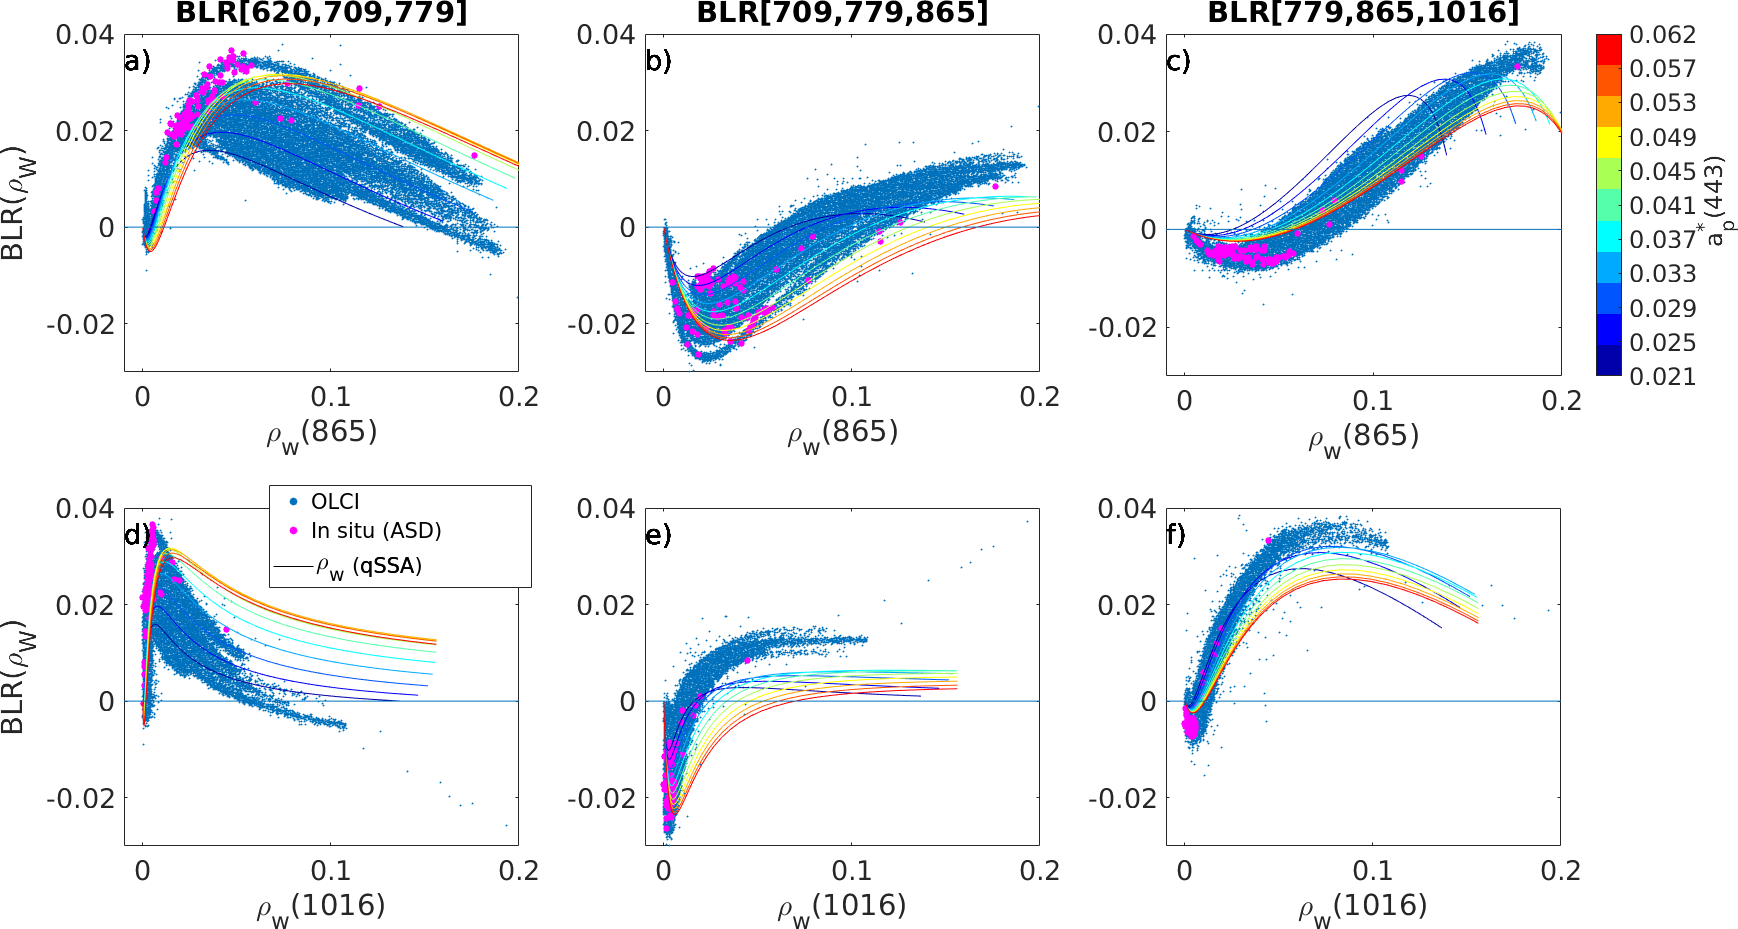
\includegraphics[width=\textwidth]{blr/figures/blrVsrhoWCalDSqSSAinSitu}
        \caption[$BLR(\rho_{w})$ en los tripletes $(620,709,779)$, $(709,779,865)$ y $(779,865,1016)$ vs. reflectancia del agua, $\rho_{w}$, en las bandas 865 nm (a-c) y 1016 nm (d-f).]{$BLR(\rho_{w})$ en los tripletes $(620,709,779)$, $(709,779,865)$ y $(779,865,1016)$ vs. reflectancia del agua, $\rho_{w}$, en las bandas 865 nm (a-c) y 1016 nm (d-f). En azul se grafican los datos extraídos de OLCI de diversas imágenes. Los puntos en magenta corresponden a mediciones radiométricas \textit{in situ}. Las líneas coloreadas corresponden a diferentes reflectancias brindadas por el modelo de Aproximación de Dispersión cuasi-Simple (qSSA, \S \ref{qssa}).}
        \label{blr:blrVsRho}
        \end{figure}
        
        Si bien existe una semejanza evidente entre las tres fuentes de información, debe notarse que las curvas qSSA se apartan de los datos medidos (tanto remótamente como \textit{in situ}) principalmente debido a que el modelo de reflectancia analítica utilizado es menos confiable a reflectancias altas debido al fuerte efecto de la dispersión múltiple a altas concentraciones de partículas.
        Las variaciones sobre la relación BLR vs. $\rho_{w}$ observadas entre las diferentes curvas qSSA indican que los BLRs pueden ser muy sensibles a la absorción de partículas; lo que significa que podrían usarse como indicativos de diferentes propiedades ópticas específicas de partículas en aguas muy turbias. No obstante, esta hipótesis debe verificarse simultáneamente con mediciones radiométricas y con datos de campo de absorción de partículas.
        
        En los tres tripletes considerados, el modelo $BLR(\rho_{w})$ se comporta de manera similar al aumentar la reflectancia. En $\rho_{w}=0$, todos se acercan a los valores cercanos a 0, recuperando el supuesto de agua negra $BLR(\rho_{w}=0)=0$ visto en la Figura \ref{blr:blrHist}. A medida que aumentan las reflectancias, los BLRs toman valores negativos, lo que se puede entender si consideramos $\rho_{w} \propto \frac{b_{b,p}^{*}}{a_{w}}$ para turbideces muy bajas (bajo contenido de sedimento) (cf. Ruddick et al. 2006, Ec. 14 \cite{ruddick2006}). Dado el modelo simple de reflectancia qSSA descrito en \S \ref{qssa}, con IOPs específicas tomadas de los valores informados en Babin et al. 2003 (a y b),\cite{babin2003a}\cite{babin2003b}, esta magnitud es convexa para las bandas OLCI consideradas, es decir, BLRs negativos (Figura \ref{blr:blrBehaviorLimits} a).
        Por el contrario, para turbideces muy altas, las reflectancias del agua tienden a alcanzar un valor constante (saturación) que depende de las IOPs específicas del contenido de partículas del agua: $\rho_{w} \propto \frac{b_{b,p}^{*}}{a_{p}^{*}+b_{b,p}^{*}}$ (cf. Dogliotti et al. 2015, Ec. A2, \cite{dogliotti2015}). En este caso, esta magnitud es cóncava para las bandas OLCI consideradas en el modelo de relfectancia qSSA, es decir, BLRs positivos (Figura \ref{blr:blrBehaviorLimits}b).
        
        \begin{figure}
        \centering
        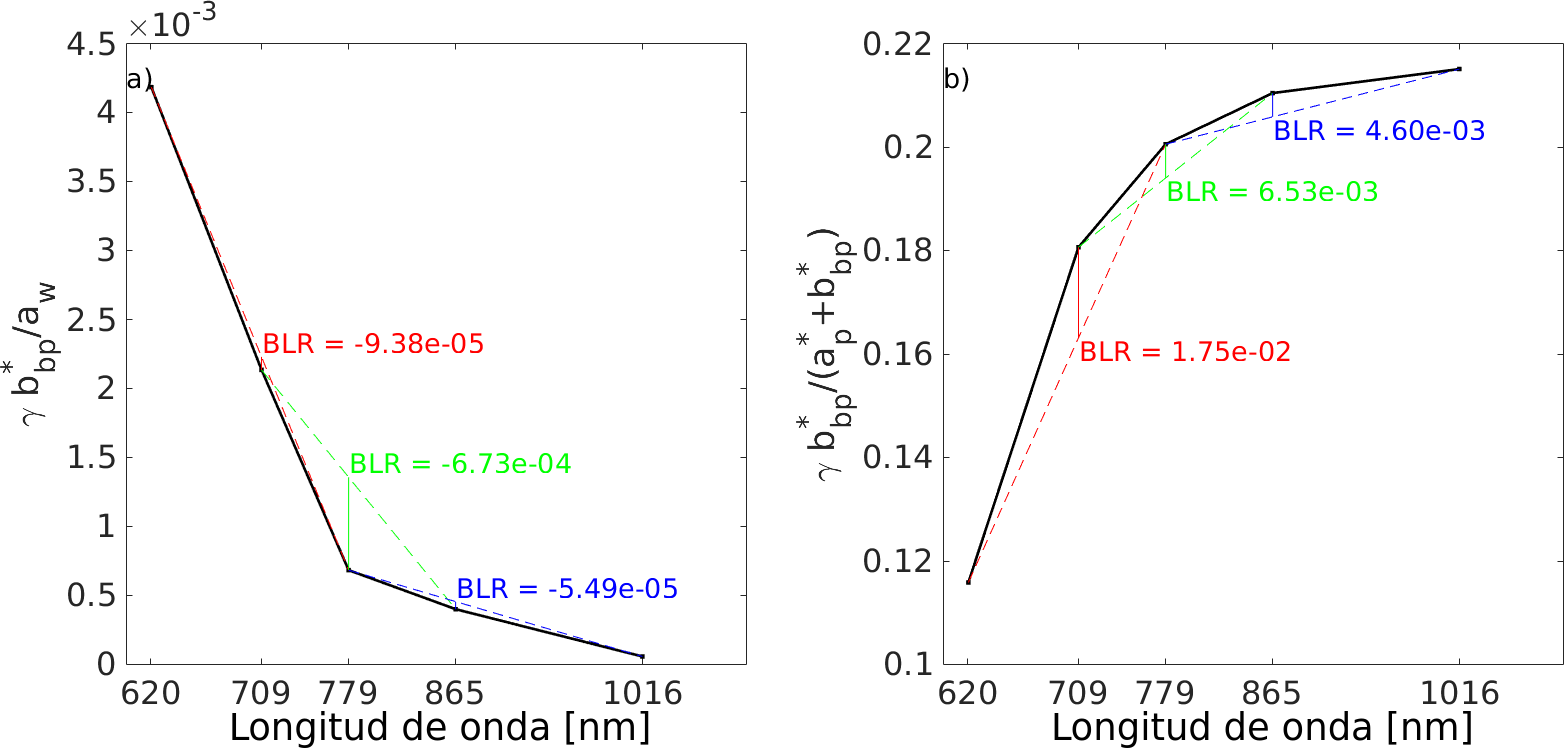
\includegraphics[width=\textwidth]{blr/figures/blrBehaviorLimits}
        \caption{Reflectancias del agua teóricas en las bandas de los BLRs otorgadas por el modelo de Aproximación de Dispersión cuasi-Simple (qSSA) a muy baja (a) y muy alta (b) concentración de partículas.}
        \label{blr:blrBehaviorLimits}
        \end{figure}

    \subsection{Efecto del ruido del sensor sobre los BLRs}
    \label{blr:s:results:blrNoise}    
        
        La Figura \ref{blr:blrQssaNoise} muestra una estimación teórica del rango de variación provocado por el ruido del sensor sobre los BLRs. Para dicha estimación se aplicaron: i) el modelo de reflectancia basado en la aproximación de Dispersión cuasi-Simple descrito en la \S \ref{qssa}; ii) los valores de error absoluto calculados mediante la aproximación de Área Homogénea, descrita en la \S \ref{blr:s:blrNoiseHA}, y la Ec. \ref{blr:eq:blrNoiseCL}.
        
            \begin{figure}
            \centering
            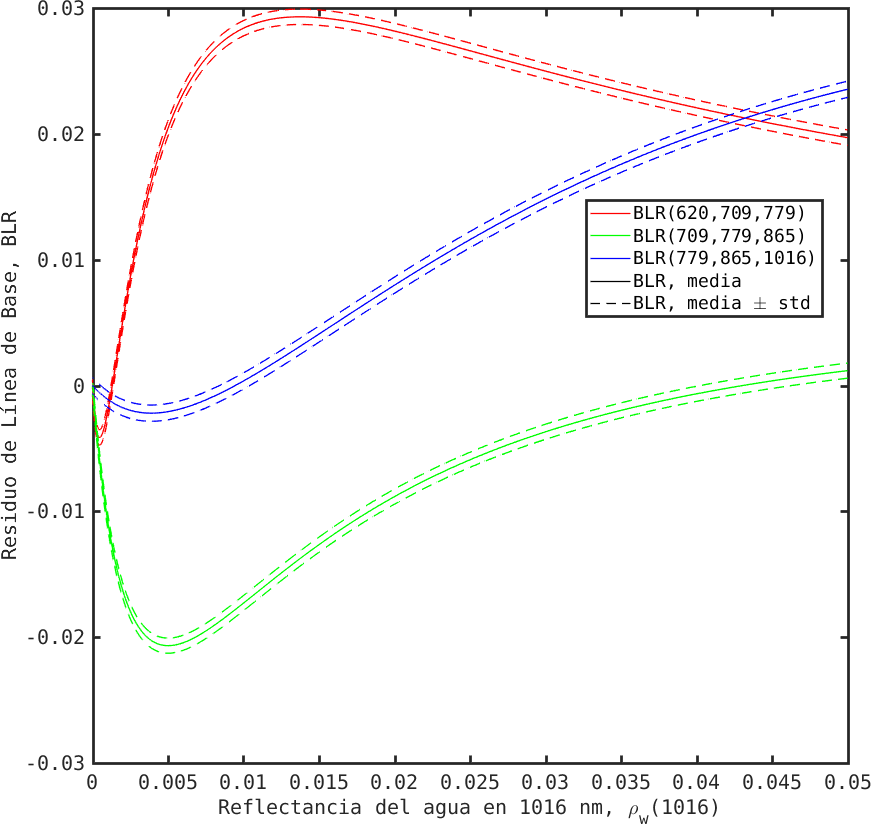
\includegraphics[width=0.7\textwidth]{blr/figures/blrQssaNoise}
            \caption[Efecto del ruido sobre los BLRs, calculado a partir del método de Área Homogénea y del modelos qSSA de reflectancia del agua.]{Valores de los BLRs considerados en este capítulo teniendo en cuenta el modelo de reflectancia del agua basado en la Aproximación de Dispersión cuasi-Simple (curvas sólidas), junto con los valores del desvío estándar del modelo teórico de error calculado a partir de la Ec. \ref{blr:eq:blrNoiseCL}.}
            \label{blr:blrQssaNoise}
            \end{figure}

        La Figura \ref{blr:blrQssaNoise} nos muestra que el efecto del ruido del sensor sobre los BLRs es suficientemente chico como para afirmar que, dadas las características del sensor considerado - OLCI-A - el mismo será capaz de resolver la forma funcional dada por la varibilidad natural de los BLRs estudiados por sobre el ruido del sensor.
        Por otro lado, la Figura \ref{blr:blrRhoRC1016Noise} muestra la reflectancia RC a 1016 nm y el $BLR(\rho_{RC})(779,865,1016)$ de una imagen OLCI-A del RdP (17 de agosto de 2016), donde se observa que el ruido de la banda a 1016 nm tiene un bajo impacto en el BLR, tal como fue detallado en la \S \ref{blr:s:blrNoise}. Más allá de estos resultados consideramos que es necesario realizar un análisis más exhaustivo del efecto del ruido del sensor sobre el desempeño de la CA.
    
        \begin{figure}
        \centering
        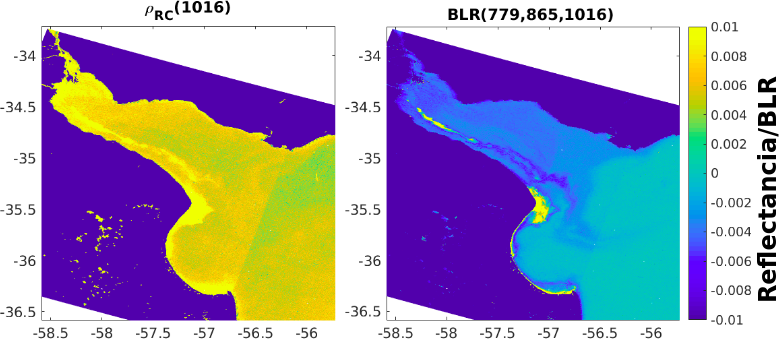
\includegraphics[width=\textwidth]{blr/figures/blrRhoRC1016Noise.png}
        \caption{Reflectancia RC a 1016 nm, $\rho_{RC}(1016)$ (a) y $BLR(\rho_{RC})[779,865,1016]$ (b) correspondientes al sensor OLCI-A sobre el Río de la Plata del día 17 de agosto de 2016.}
        \label{blr:blrRhoRC1016Noise}
        \end{figure}

    \subsection{Desempeño de la corrección atmosférica}
    \label{blr:s:results:blrac}

        \subsection{Validación con datos \textit{in situ} (\textit{match-ups})}
        \label{blr:s:results:blrac:matchups}

            Las Figuras \ref{blr:matchups_rho_hyper}, \ref{blr:matchups_rho_scatter}, \ref{blr:matchups_rho_MAE} y \ref{blr:matchups_T} muestran los resultados obtenidos para el ejercicio de \textit{match-up} realizado sobre las mediciones de las estaciones del Cuadro \ref{blr:tab:matchups} (Dogliotti y Gossn 2019, \cite{dogliottiGossn2019}). La Figura \ref{blr:matchups_rho_hyper} muestra las reflectancias del agua medidas \textit{in situ} (líneas sólidas) y los valores de reflectancia del agua obtenidos al aplicar diferentes CAs entre las que se halla la propuesta en este capítulo (denominada con el acrónimo BLR-AC). Cabe resaltar que en este ejercicio de intercomparación se consideraron únicamente bandas en el RNS para el esquema BLR-AC, es decir que no fue considerado aún en este análisis un esquema de extrapolación a bandas por debajo de 600 nm. 
            
            Se observa de las Figuras \ref{blr:matchups_rho_hyper} y \ref{blr:matchups_rho_scatter} que la correspondencia entre los datos medidos y los estimados por BLR-AC es generalmente muy buena en comparación con los esquemas restantes considerados. En particular, se observan para BLR-AC los valores de MAE más bajos en las bandas de $620$, $709$, $779$ y $865$ nm (Figura \ref{blr:matchups_rho_MAE}), seguido de la corrección estándar de los productos L2 de OLCI (BAC/BPAC). Los resultados de esta última CA en conjunto con BLR-AC son los que más se asemejan a la forma funcional de los espectros medidos \textit{in situ}. Por otro lado, en el caso de las CAs basadas en redes neuronales, C2RCC y C2RCCnewNN, se observan en general mayores discrepancias con los datos medidos \textit{in situ}, con una marcada subestimación de la reflectancia en todo el espectro en la estación RdP\_20170106\_M0117-02 en el caso de C2RCC; una marcada subestimación en la estación RdP\_20181105\_PTG-P13 en el caso de C2RCCnewNN (la cual subestima las reflectancias en la región violeta/azul en todos los casos). En la región RNS, BLR-AC es la que mejor estima la reflectancia del agua en todas las estaciones a excepción de RdP\_20170126\_test1 donde tiende a sobreestimar los valores en el rojo, al igual que BAC/BPAC.
    
            \begin{figure}
            \centering
            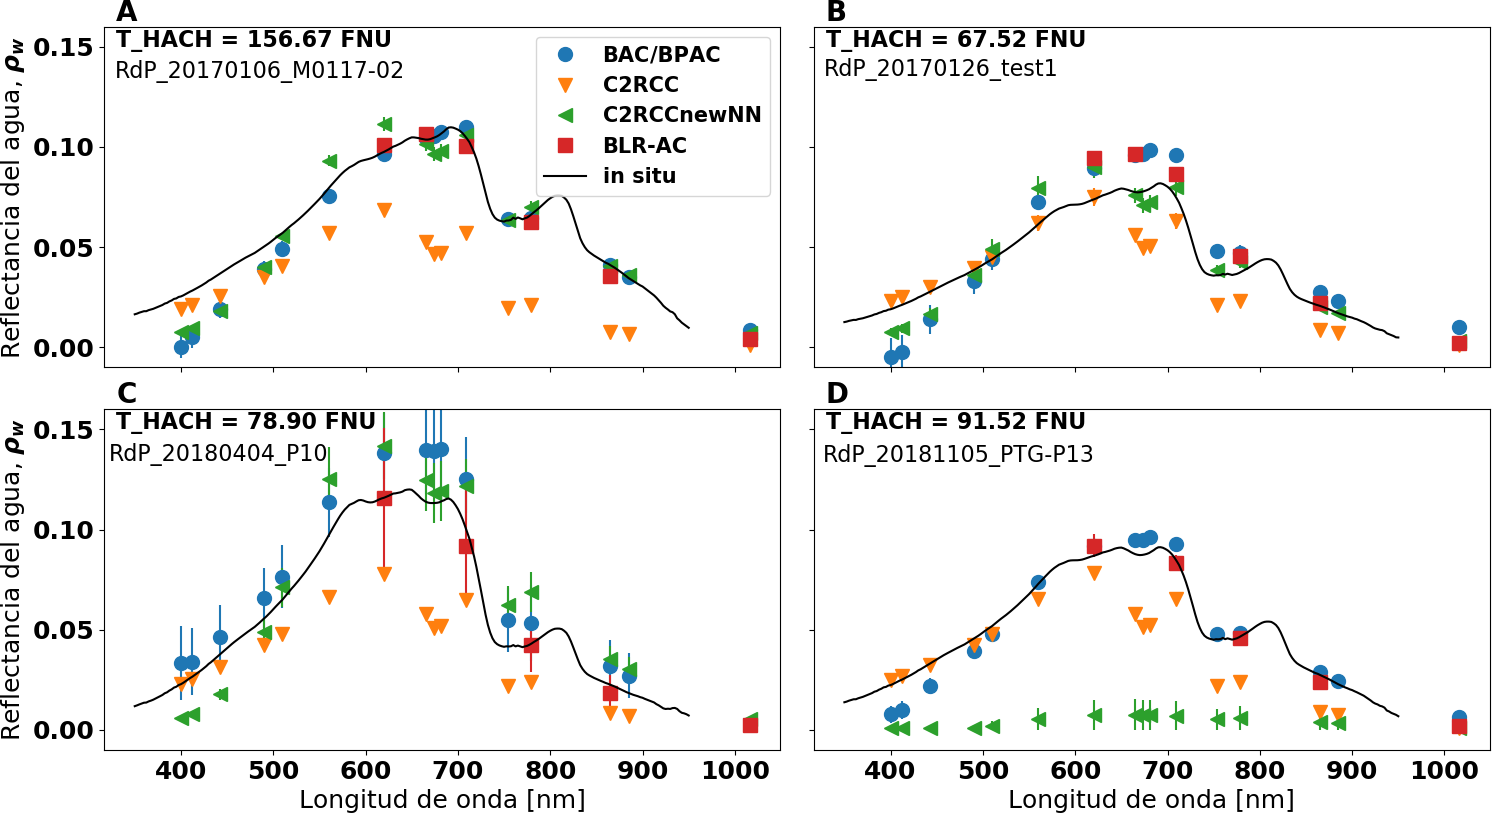
\includegraphics[width=\textwidth]{blr/figures/matchups_rho_hyper.png}
            \caption[Reflectancias del agua medidas \textit{in situ} y estimadas a partir de imágenes OLCI y de diferentes esquemas de corrección atmosférica (BLR-AC, BAC/BPAC, C2RCC y C2RCCnewNN) para las estaciones detalladas en el Cuadro \ref{blr:tab:matchups}]{Reflectancias del agua medidas \textit{in situ} (hiperespectrales, líneas negras sólidas) y estimadas a partir de imágenes OLCI y de diferentes esquemas de corrección atmosférica (BLR-AC, BAC/BPAC, C2RCC y C2RCCnewNN) para las estaciones detalladas en el Cuadro \ref{blr:tab:matchups}. Las barras de error fueron estimadas a partir del desvío estándar de $\rho_{w}$ sobre las ventanas de $3 px \times3 px$ utilizadas para los \textit{match-ups}. Se indican también los valores de turbidez medidos por el turbidímetro portátil HACH para cada estación (\S \ref{dat:s:hach}).}
            \label{blr:matchups_rho_hyper}
            \end{figure}
            
            \begin{figure}
            \centering
            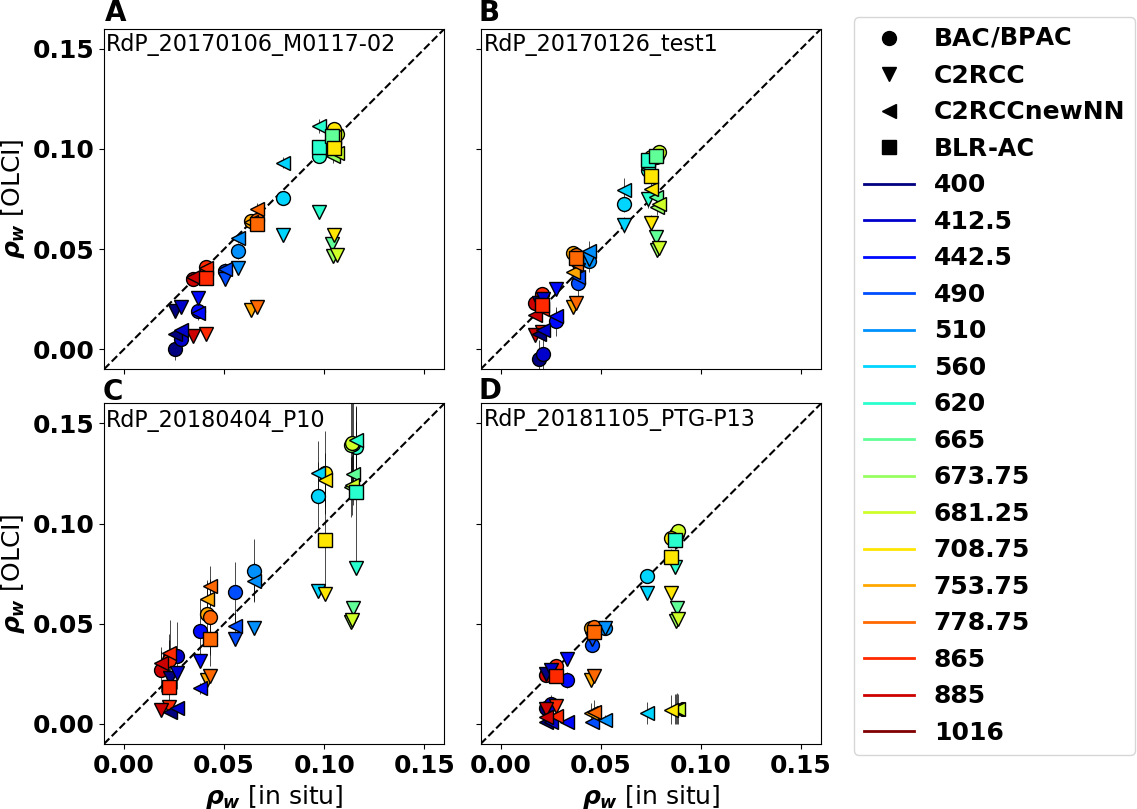
\includegraphics[width=\textwidth]{blr/figures/matchups_rho_scatter.png}
            \caption[Reflectancias del agua estimadas a partir de imágenes OLCI (CAs BLR-AC, BAC/BPAC, C2RCC y C2RCCnewNN) vs. reflectancias del agua medidas \textit{in situ}.]{Reflectancias del agua estimadas a partir de imágenes OLCI (CAs BLR-AC, BAC/BPAC, C2RCC y C2RCCnewNN) vs. reflectancias del agua medidas \textit{in situ}. Las formas de los símbolos representan diferentes esquemas, y la escala de colores varía según la banda OLCI considerada.}
            \label{blr:matchups_rho_scatter}
            \end{figure}
            
            \begin{figure}
            \centering
            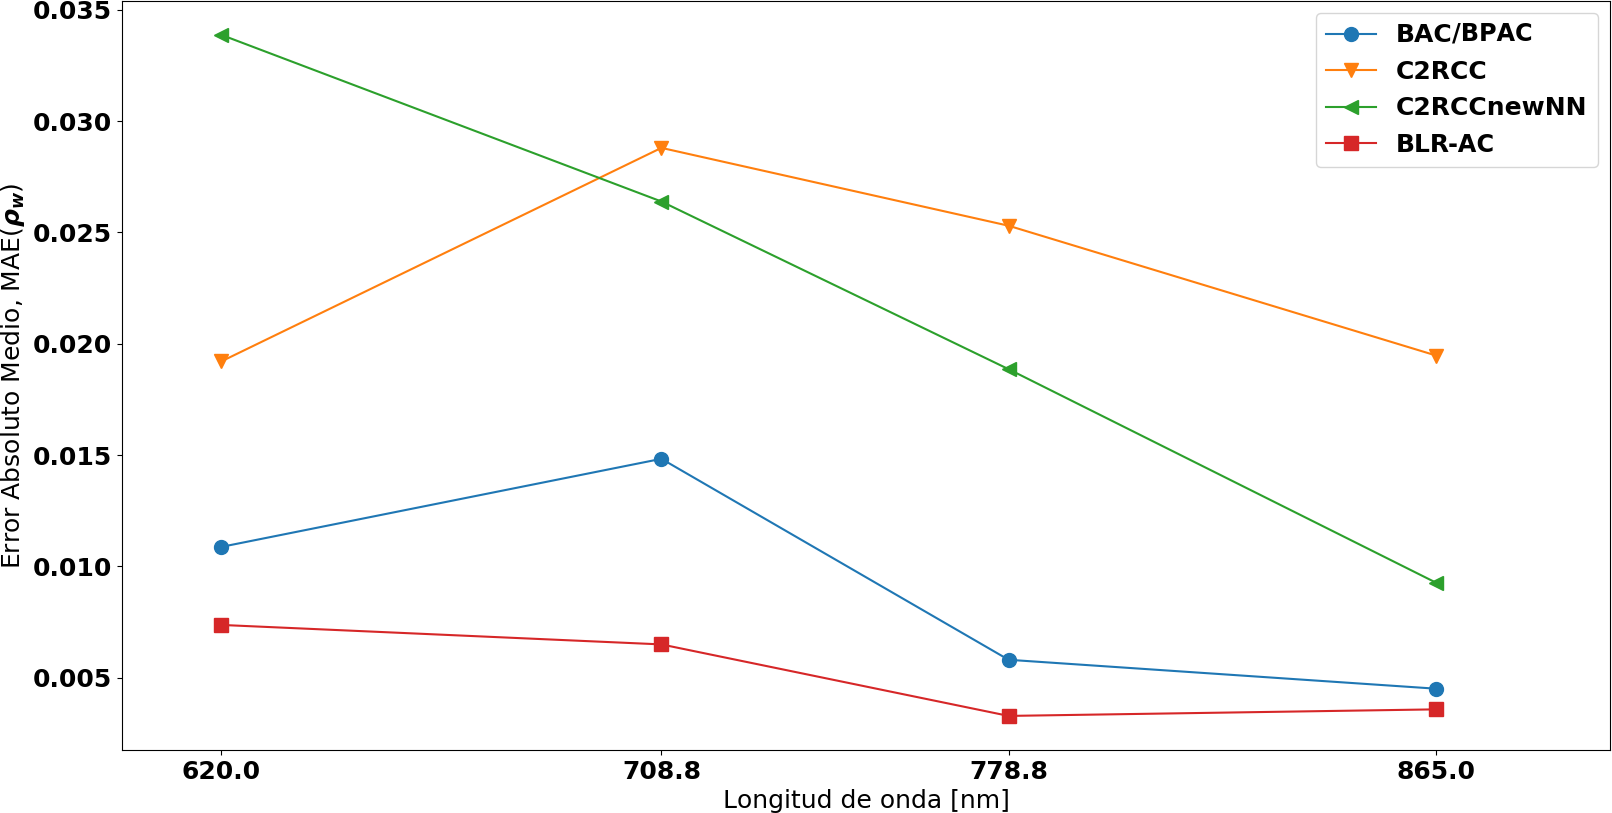
\includegraphics[width=\textwidth]{blr/figures/matchups_rho_MAE.png}
            \caption[Errores absolutos medios calculados sobre las 4 estaciones en las que se efectuó el ejercicio de \textit{match-up} para las bandas 620, 709, 779 y 865 1016 nm.]{Errores absolutos medios (MAEs, Ec. \ref{blr:eq:MAE}) calculados sobre las 4 estaciones en las que se efectuó el ejercicio de \textit{match-up} (Cuadro \ref{blr:tab:matchups}) para las bandas 620, 709, 779 y 865 1016 nm.}
            \label{blr:matchups_rho_MAE}
            \end{figure}
            
            Por otro lado, la Figura \ref{blr:matchups_T} compara los valores estimados por las diferentes CAs y los valores obtenidos \textit{in situ} de la turbidez del algoritmo de Dogliotti et al. 2015 (\S \ref{dat:s:dog15}) a partir de la banda de OLCI en $865$ nm (es decir, asumiendo un parámetro de trancisión del rojo al NIR de $\omega=1$, Ec. \ref{dat:eq:dogliotti2015}). Nuevamente, se observa una mejor correspondencia entre la estimación y la observación para el algoritmo de BLR-AC, con un valor de MAE de $19.71 FNU$, siendo los valores de MAE obtenidos para el resto de las CAs de $24.06 FNU$ (BAC/BPAC), $46.76 FNU$ (C2RCCnewNN) y $97.48 FNU$ (C2RCC). Naturalmente, dicha correspondencia entre turbideces observada y estimada a partir de BLR-AC es concomitante con los buenos resultados obtenidos en la región del NIR para este esquema.
            
            \begin{figure}
            \centering
            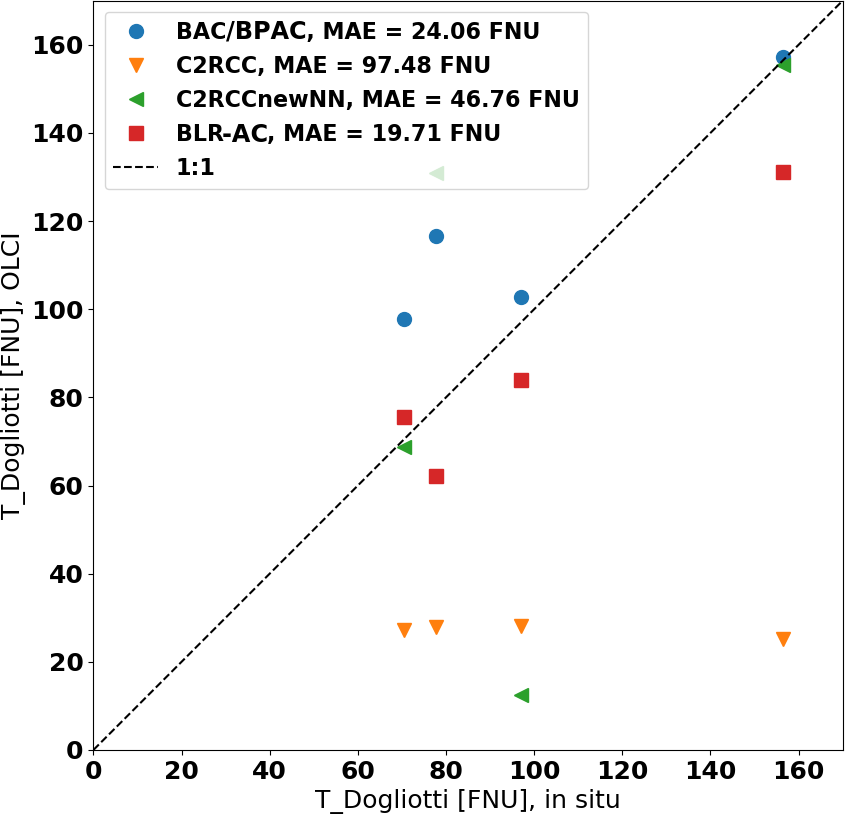
\includegraphics[width=0.65\textwidth]{blr/figures/matchups_T.png}
            \caption[Turbidez (Dogliotti et al. 2015) estimada a partir de reflectancias del agua de imágenes OLCI - utilizando los esquemas BLR-AC, BAC/BPAC, C2RCC y C2RCCnewNN - vs. estimada a partir de la reflectancia del agua medida \textit{in situ}.]{Turbidez estimada a partir de reflectancias del agua de imágenes OLCI - utilizando los esquemas BLR-AC, BAC/BPAC, C2RCC y C2RCCnewNN - vs. estimada a partir de la reflectancia del agua medida \textit{in situ}. El algoritmo de turbidez utilizado es el de Dogliotti et al. 2015 (\S \ref{dat:s:dog15}).}
            \label{blr:matchups_T}
            \end{figure}

        \subsection{Validación a partir del esquema Fix-AC}
        \label{blr:s:results:blrac:fixac}
        
            Dada la falta de suficientes \textit{match-ups} entre las mediciones \textit{in situ} y los datos OLCI para el Río de la Plata, el enfoque Fix-AC (considerado de alto rendimiento para las escenas elegidas pero no apropiado para un procesador global automatizado) se utilizó como referencia para validar el rendimiento del esquema BLR-AC (Figura \ref{blr:ACInterFixAC}). Se seleccionaron los píxeles dentro de los rectángulos de colores marcados, correspondientes a las partes más turbias de las imágenes de validación enumeradas en el Cuadro \ref{blr:tab:olci}. Las tres regiones se seleccionaron como representativas de aguas extremadamente turbias (Figura \ref{blr:ACInterFixAC} b) y moderadamente turbias (Figura \ref{blr:ACInterFixAC} a, c). Las reflectancias del agua derivadas de ambos enfoques muestran patrones muy similares y valores de RMSD (Ec. \ref{blr:eq:RMSD}) muy pequeños en ambos casos.
            En el caso de la banda de 620 nm, los valores de $\rho_{w}^{BLR-AC}$ se obtuvieron mediante el uso de una extrapolación lineal simple de la señal de aerosoles de las bandas de corrección de 865 nm y 1016 nm.

            \begin{figure}
            \centering
            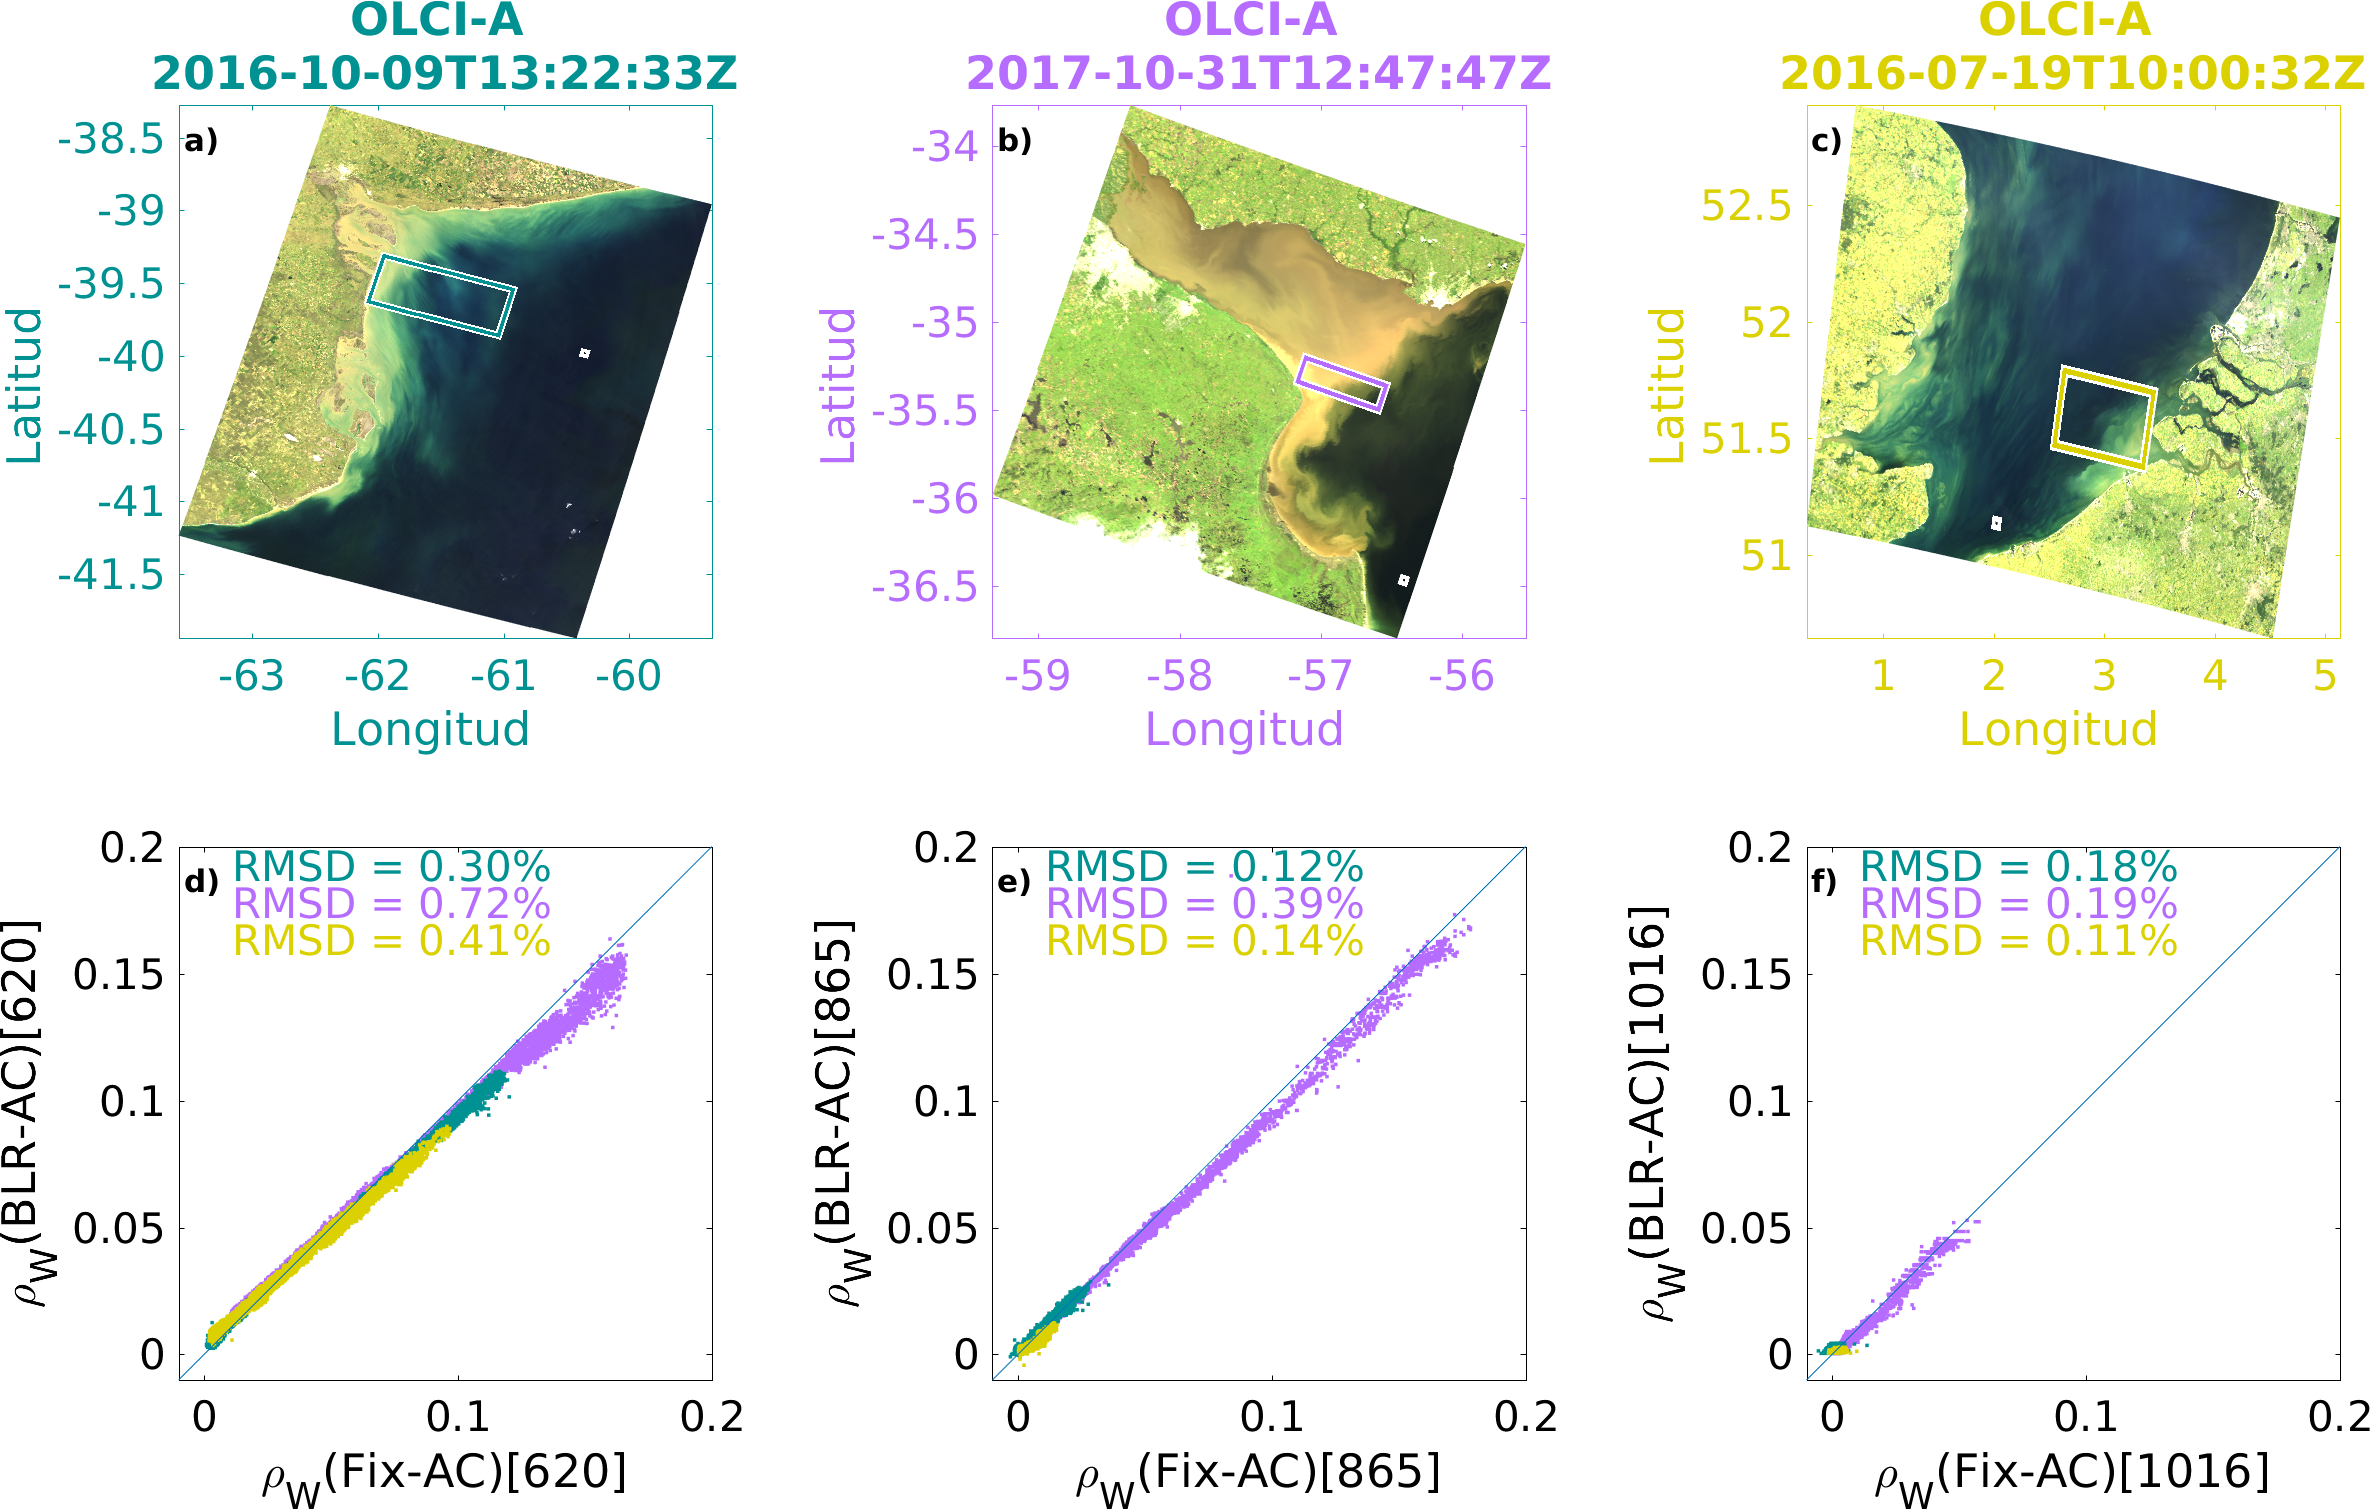
\includegraphics[width=\textwidth]{blr/figures/ValFixAcVsBlrAc}
            \caption[Intercomparación entre esquemas BLR-AC y Fix-AC.]{Intercomparación entre esquemas BLR-AC y Fix-AC. Composiciones RGB de escenas de las regiones de Bahía Blanca (ARG), Río de la Plata y Costa belga de donde se adquirieron los conjuntos de datos (cuadros turquesa, violeta y amarillo ocre en los recuadros a-c, resp.). Las reflectancias del agua otorgadas por BLR-AC y Fix-AC, $\rho_{w}^{BLR-AC}$ y $\rho_{w}^{Fix-AC}$ se comparan para los recuadros seleccionados en las bandas 620 nm (d), 865 nm (e) y 1016 nm ( F). Los valores de $\rho_{w}^{BLR-AC}(620)$ se estimaron por extrapolación lineal simple de la reflectancia del aerosoles de 865 nm y 1016 nm.}
            \label{blr:ACInterFixAC}
            \end{figure}

        \subsection{Correlación espacial entre reflectancias del agua y de aerosoles}
        \label{blr:s:results:blrac:correlacionEspacial}
        
            Otra forma de evaluar el rendimiento de una corrección atmosférica es a través del análisis de la (de-)correlación espacial entre las reflectancias estimadas del agua y de aerosoles. Las Figuras \ref{blr:ACInter1} - \ref{blr:ACInter3} muestran reflectancias del agua y de aerosoles a 1016 nm brindadas por la BLR-AC para diferentes escenas de OLCI sobre el Río de la Plata (2017-01-21T13:24:42Z,2016-06-08T13:09:51Z, 2017-12-12T12:59:01Z, Cuadro \ref{blr:tab:olci}), junto con los valores otorgados por correcciones atmosféricas estándar: BAC/BPAC de la ESA y SeaDAS-2 de la NASA(865,1016) (\S \ref{blr:s:olci}). La región más difícil para la corrección atmosférica sobre el RdP es el frente de turbidez adyacente a la costa de la provincia de Buenos Aires (Argentina) a alrededor de $35 \degree0 S; \, \, 57 \degree0 W$ (marcado como $0.8 \degree \times 0.8 \degree$ recuadros negros, \S \ref{int:s:area}), donde los valores de SPM, turbidez y reflectancias del agua en el RNS son máximas \cite{framinan1996}\cite{dogliotti2011}. Es evidente a partir de las pendientes más altas y los valores $R^{2}$ obtenidos para las regresiones lineales en la Figura \ref{blr:ACInter1}b-c cómo las correcciones atmosféricas estándar producen una correlación más alta (no física) entre las señales del agua y de aerosoles. Esto también es evidente al comparar visualmente los \textit{rasters} de agua y aerosoles en el caso BLR-AC, en comparación con BAC/BPAC y SeaDAS-2(865,1016). En términos generales, BAC/BPAC y SeaDAS-2(865,1016) subestiman la señal de agua o simplemente no convergen a una solución numérica (es decir, producen valores NaN, \textit{Not-a-Number}, marcados en magenta en las Figuras \ref{blr:ACInter1} - \ref{blr:ACInter3} e, f, h, i). La imagen que se muestra en la Figura \ref{blr:ACInter1} está parcialmente contaminada con \textit{sunglint} moderado (hacia el borde Este), que se considera como señal que no es agua para los esquemas BLR-AC y BAC/BPAC. La imagen que se muestra en la Figura \ref{blr:ACInter3} está parcialmente contaminada con nubes delgadas. En este caso se observa cómo BLR-AC es claramente capaz de separar la nube delgada de la señal de agua turbia.
    
            \begin{figure}
            \centering
            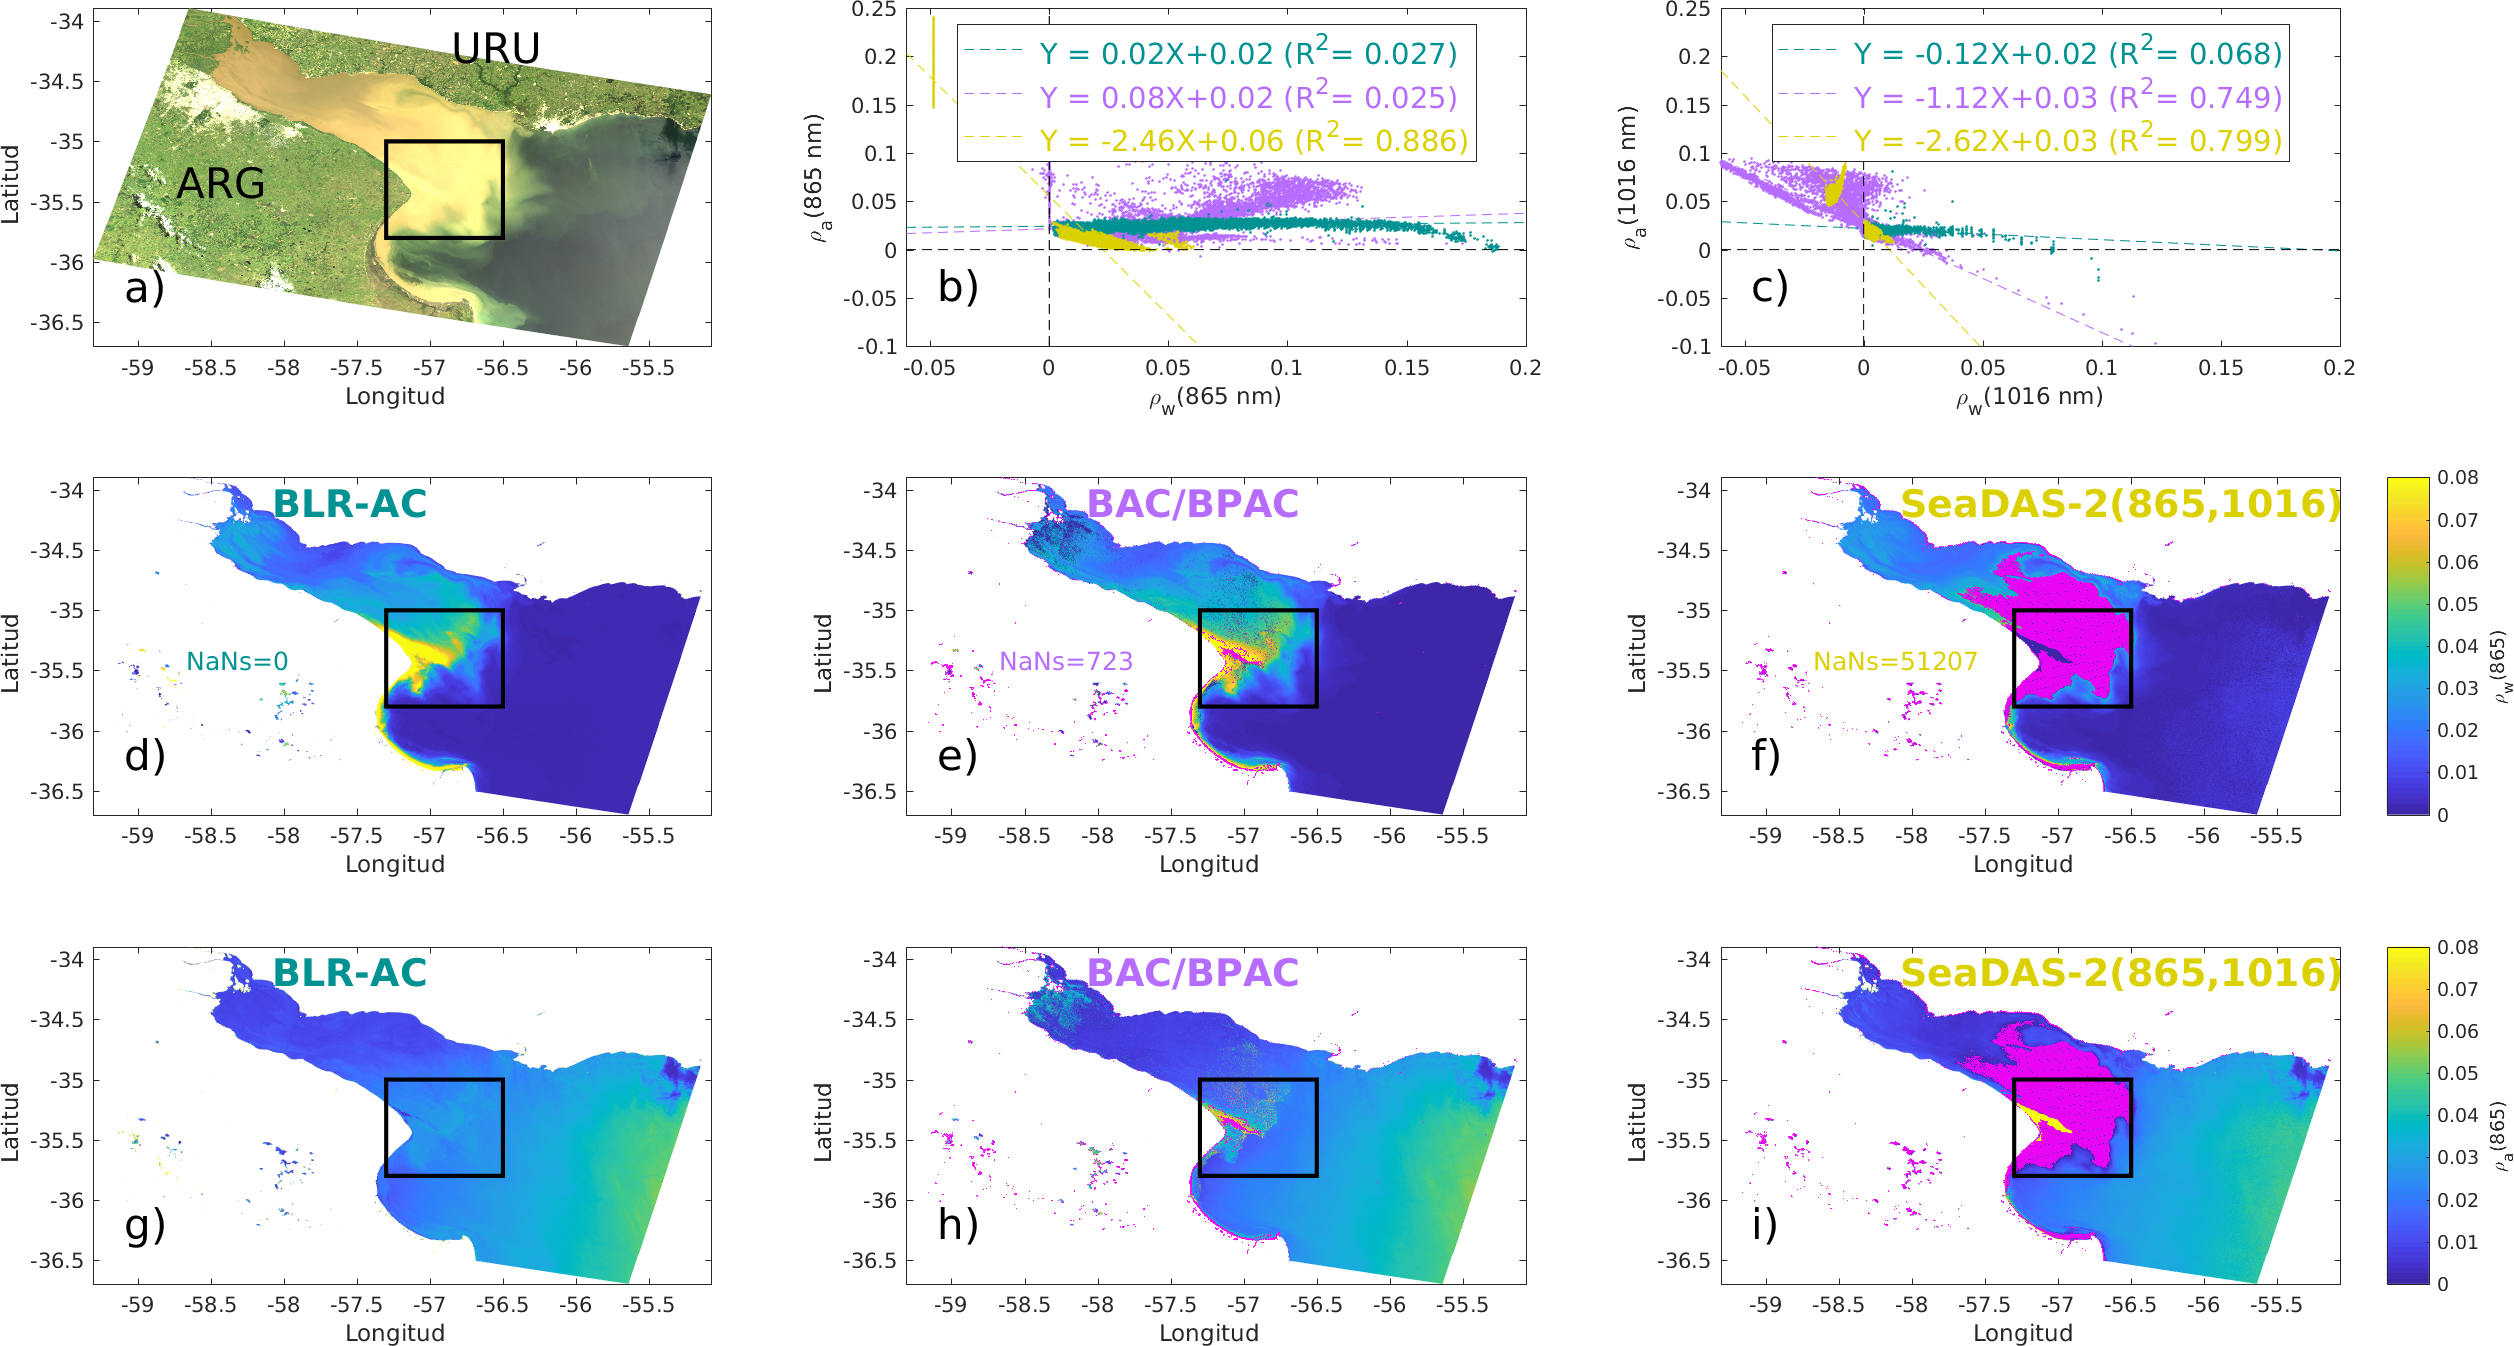
\includegraphics[width=\textwidth]{blr/figures/ACInter1.png}
            \caption[Comparación entre esquemas de CA: BLR-AC, BAC/BPAC y SeaDAS-2(865,1016) aplicados sobre una imagen OLCI-A adquirida en 2017-01-21T13:24:42Z sobre el Río de la Plata.]{Comparación entre esquemas de CA: BLR-AC, BAC/BPAC y SeaDAS-2(865,1016) aplicados sobre una imagen OLCI-A adquirida en 2017-01-21T13:24:42Z sobre el Río de la Plata. a): Composición RGB. b)-c): Reflectancias del agua vs. de aerosoles a 865/1016 nm sobre la subregión del frente de turbidez (demarcada con rectángulos negros). d)-i): Reflectancia del agua y de aerosoles en 865 nm, estimada por: BLR-AC (d,g), la CA estándar de OLCI (BAC/BPAC) (e,h) y el procedimiento iterativo de SeaDAS utilizando las bandas 865 nm y 1016 nm (SeaDAS-2(865,1016)) (f,i). Los píxeles donde las CAs fallaron (NaNs) están marcados en magenta.}
            \label{blr:ACInter1}
            \end{figure}
            
            \begin{figure}
            \centering
            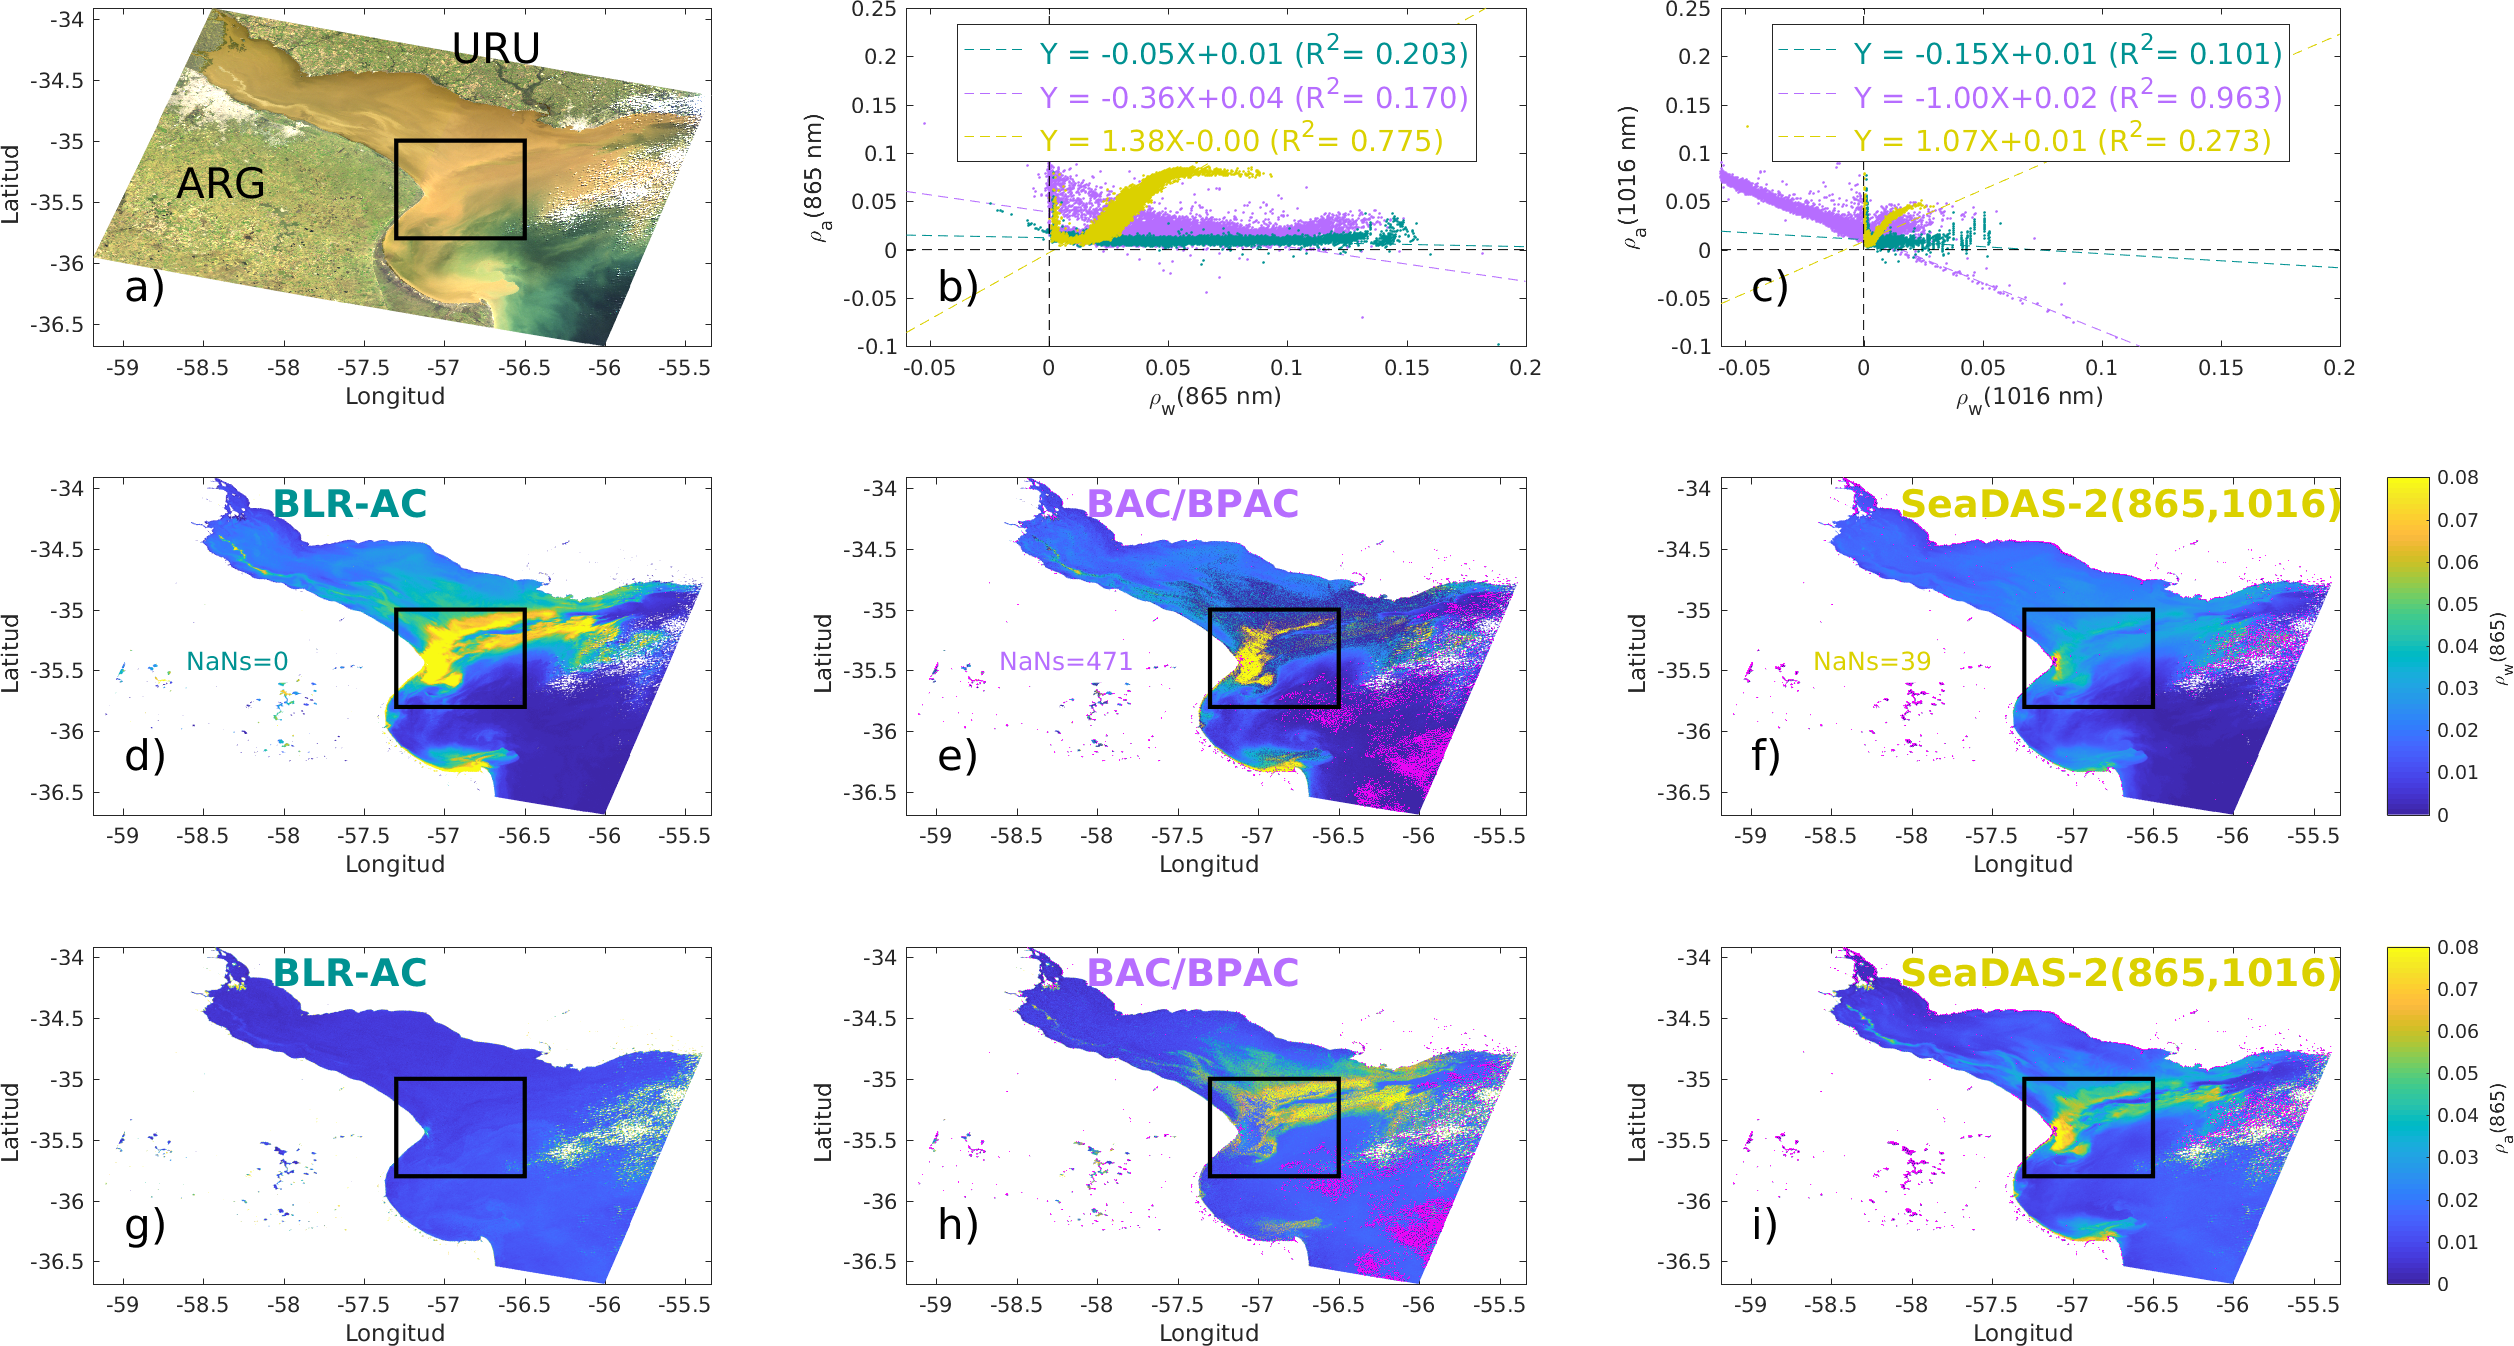
\includegraphics[width=\textwidth]{blr/figures/ACInter2.png}
            \caption{Ídem \ref{blr:ACInter1}, pero para 2016-06-08T13:09:51Z.}
            \label{blr:ACInter2}
            \end{figure}
            
            \begin{figure}
            \centering
            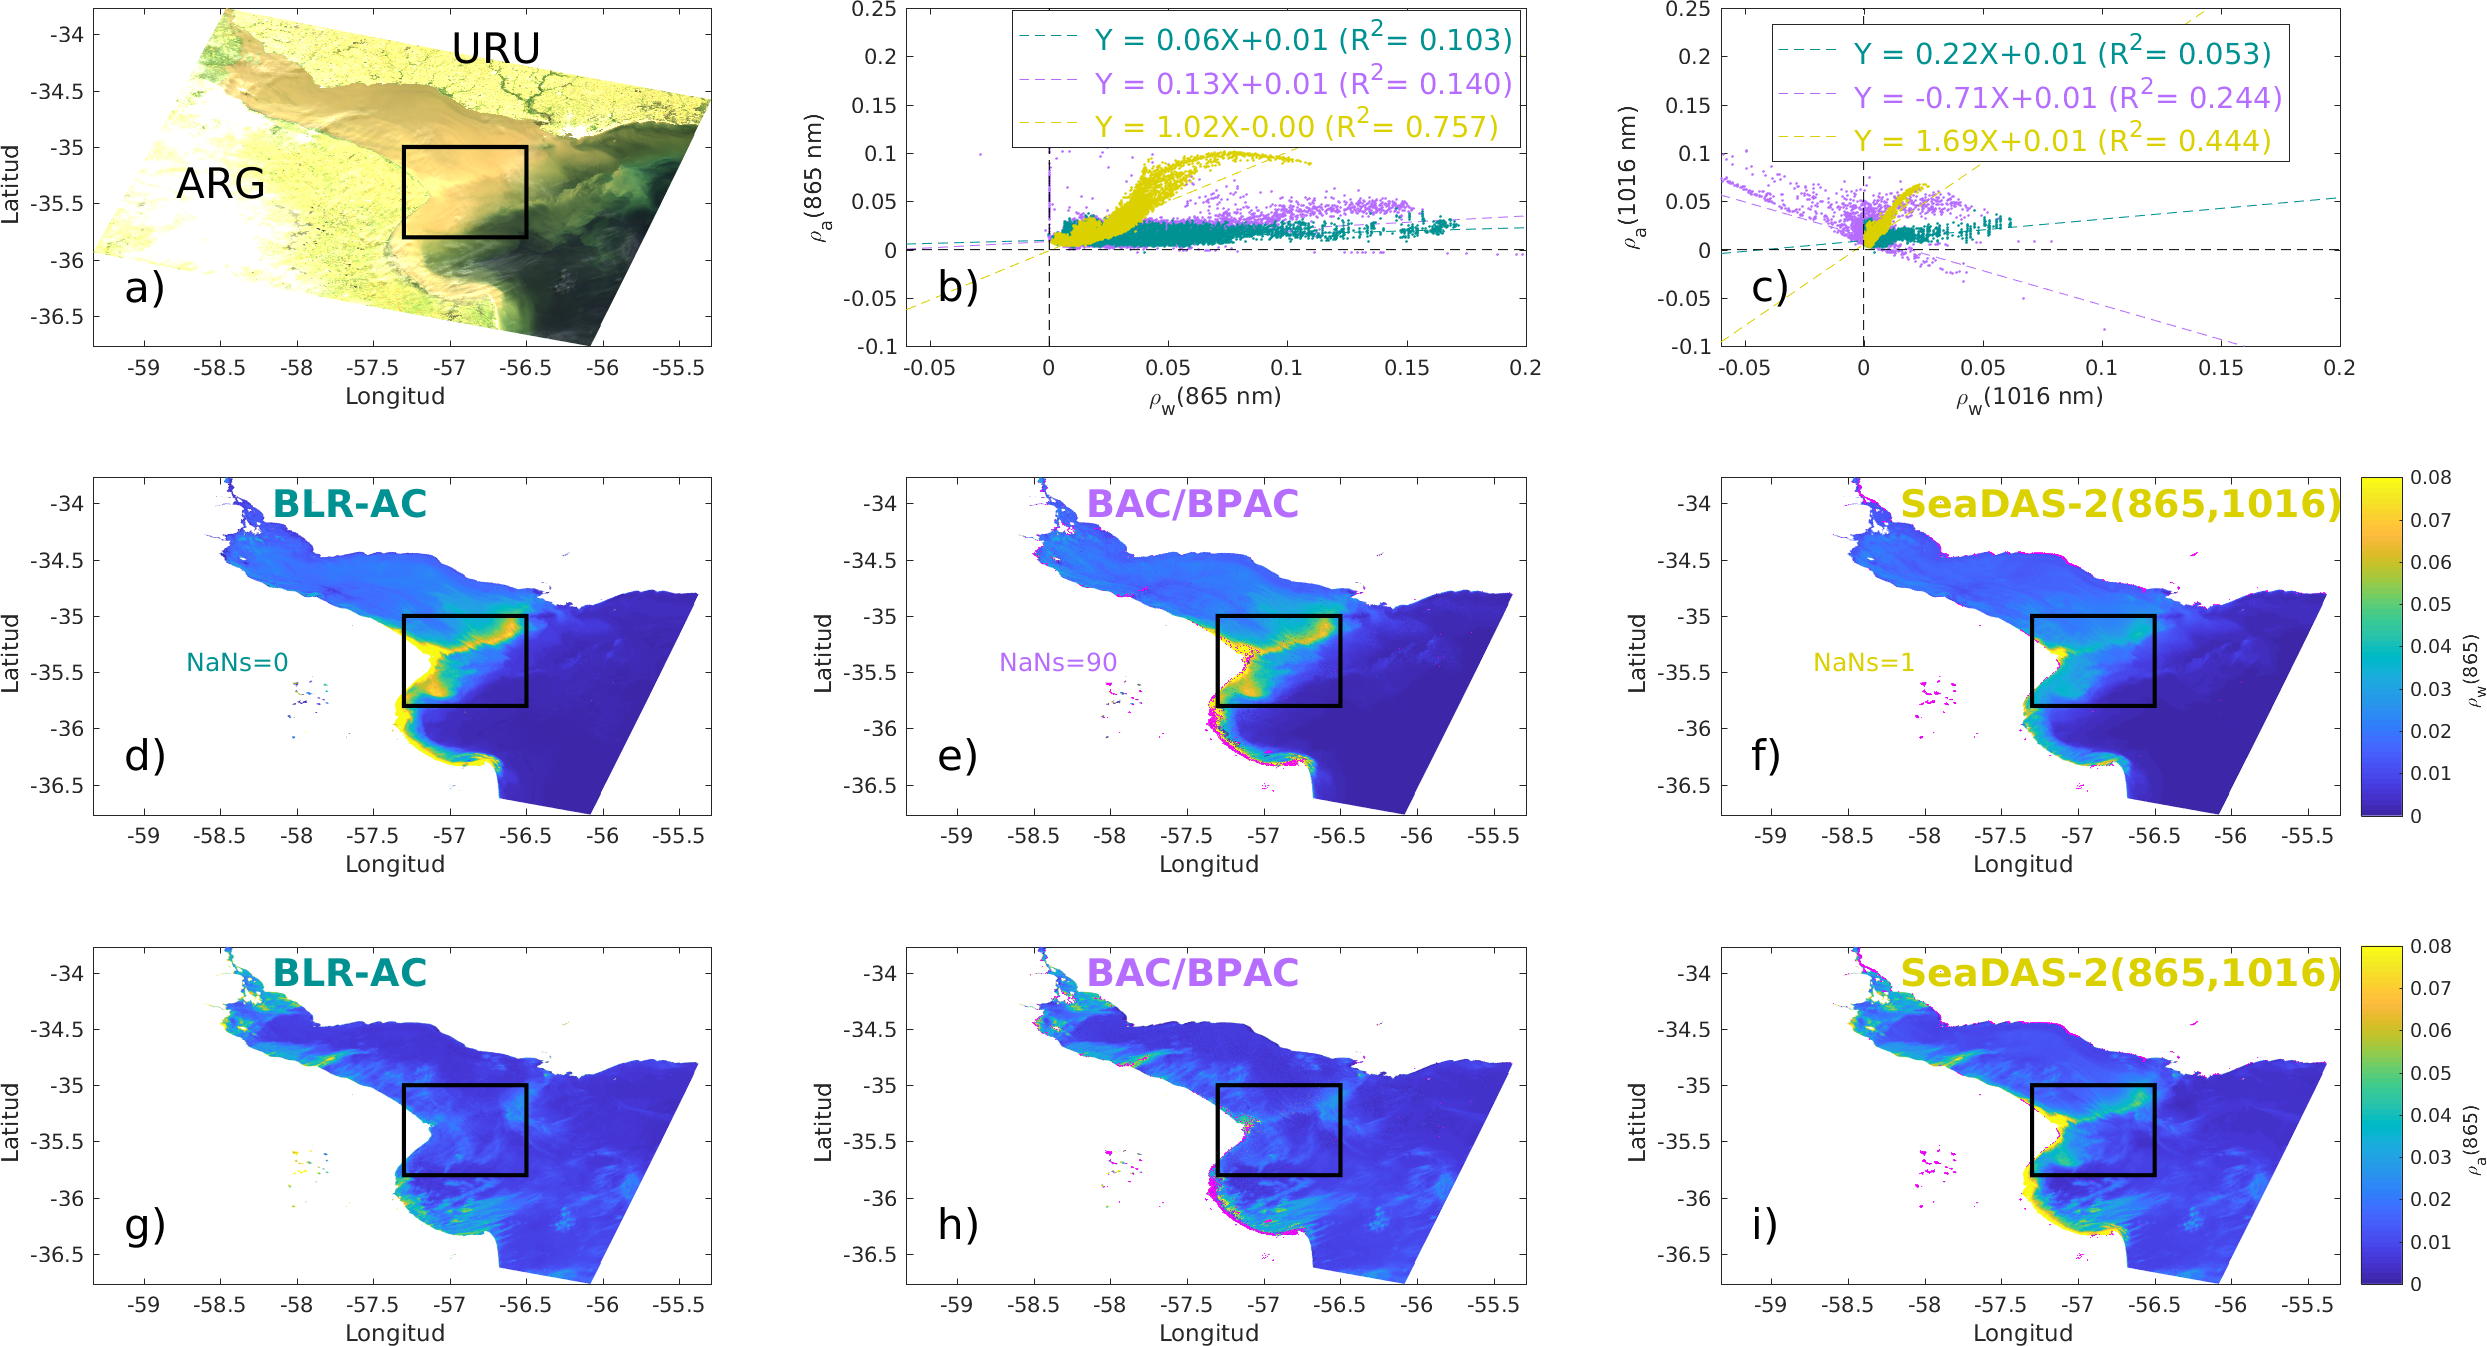
\includegraphics[width=\textwidth]{blr/figures/ACInter3.png}
            \caption{Ídem \ref{blr:ACInter1}, pero para 2017-12-12T12:59:01Z.}
            \label{blr:ACInter3}
            \end{figure}

%%%%%%%%%%%%%%%%%%%%%%%%%%%%%%%%%%%%%%%%%%
\section{Discusión}
\label{blr:s:discussion}

    El nuevo enfoque de CA presentado aquí tiene la ventaja de que está diseñado sobre la base de principios físicos claros y, por lo tanto, permite comprender (e.g., Figura \ref{blr:blr3d}) cómo factores como la variabilidad natural de las propiedades ópticas inherentes específicas del agua, la calibración a TOA de datos satelitales y la elección de bandas espectrales pueden afectar el rendimiento del algoritmo. Los BLRs calculados a partir de mediciones \textit{in situ} y los datos OLCI se comportan de manera similar y de acuerdo con un modelo de reflectancia de Aproximación de Dispersión cuasi-Simple (qSSA), aunque el modelo qSSA no tiene un buen desempeño para reflectancias medidas en regímenes de turbidez extrema, debido a la vulneración de las aproximaciones subyacentes al modelo qSSA (Figura \ref{blr:blrVsRho}).
    
    Si bien el nuevo algoritmo ya muestra un buen desempeño en la estimación de la reflectancia en el agua en el Rojo/NIR/SWIR, particularmente en aguas extremadamente turbias, y por lo tanto puede usarse directamente para la estimación de la turbidez, SPM y concentración de clorofila-a (en aguas turbias utilizando algoritmos Rojo/NIR), son necesarias mejoras adicionales para la estimación de la reflectancia del agua a longitudes de onda más cortas si es que estas últimas bandas espectrales son eventualmente requeridas para la estimación de otros productos biogeofísicos satelitales.
    
    En aguas extremadamente turbias, la reflectancia corregida por Rayleigh en el Rojo/NIR está dominada por las reflectancias del agua y de aerosoles estimadas y, en particular, el tipo de aerosol estimado (a través de $\epsilon_{a}(865,1016)$) puede verse muy afectado por pequeños errores en las estimaciones de reflectancias del agua. De hecho, en esta situación (de aguas muy turbias), es precisamente la reflectancia del agua la que se puede estimar mejor en términos relativos que la reflectancia de aerosoles. Si bien se requieren valores de $\epsilon_{a}(865,1016)$ más confiables en aguas extremadamente turbias para la extrapolación a longitudes de onda más cortas, entonces el enfoque actual podría mejorarse en el futuro mediante la integración de información adicional. Por ejemplo, se podrían aplicar restricciones adicionales a $\epsilon_{a}(865,1016)$ mediante el uso de bandas en el ultravioleta/violeta (mediante la correcta demostración e implementación del supuesto de anclaje en el violeta, \S \ref{int:s:ACUV}) o mediante el suavizado espacial de $\epsilon_{a}(865,1016)$ suponiendo que la escala de longitud horizontal para la variación del tipo de aerosol es mayor que el tamaño de píxel (Ruddick et al. 2000, \cite{ruddick2000}). En el presente capítulo no se ha aplicado dicha suavización horizontal, lo que nos permite comprender mejor las capacidades y limitaciones de un enfoque automatizado de píxel a píxel y, por lo tanto, identificar, por ejemplo, el valor intrínseco de las diversas bandas espectrales en la separación de las señales de aerosol y agua en el RNS y las posibles fuentes de incertidumbre en esta descomposición. En una versión futura del algoritmo, la restricción sobre $\epsilon_{a}(865,1016)$ aplicada en el último paso (\S \ref{blr:s:summary}, paso 7) del procesamiento podría reemplazarse por restricciones tanto espectrales como espaciales, y se podría abordar la optimización BLR con un método más refinado.
    
    Si bien el nuevo algoritmo se basa en una superficie de calibración BLR construida con imágenes OLCI del Río de la Plata (\S \ref{blr:s:summary}, paso 5), el esquema de CA también se ha probado en muchos otros sitios con aguas dominadas por sedimentos, como la Pluma de Amazonas en el Atlántico, Mar de Bohai, Costa belga, Bahía Blanca (Delgado et al. 2018, \cite{delgado2018}) y el Río Girondo (Renosh et al. (enviado), \cite{renosh2019}), utilizando esta superficie de calibración, por lo que actualmente consideramos que no sería necesario aplicar diferentes calibraciones a diferentes regiones.

\section{Conclusiones}
\label{blr:s:conclusion}

    En este capítulo de la tesis se presentó un nuevo algoritmo de CA para aguas extremadamente turbias para el sensor S3/OLCI. La suposición clave es que la convexidad espectral de la reflectancia corregida por Rayleigh en el RNS está determinada por la reflectancia del agua y no se ve esencialmente afectada por los aerosoles. Esta convexidad espectral se cuantifica aquí a través de los Residuos de la Línea de Base (BLRs, Ec. \ref{blr:eq:blr}) de los tres tripletes consecutivos de las bandas OLCI centradas en 620, 709, 779, 865 y 1016 nm. Una transmitancia equivalente aplicable a los BLRs que depende del factor geométrico de masa de aire se derivó de mediciones \textit{in situ} y simulaciones de transferencia radiativa. El algoritmo que relaciona los BLRs con las reflectancias del agua a 865 y 1016 nm se calibró utilizando datos OLCI de subregiones seleccionadas de imágenes del Río de la Plata, que fueron corregidas atmosféricamente mediante un esquema simple de ventana fija (Fix-AC) que supone la homogeneidad espacial de la atmósfera (dadas las condiciones de cielo muy despejado y distancias horizontales pequeñas a la ventana fija) y calcula la reflectancia atmosférica de las ventanas fijas correspondientes a las regiones de aguas claras. El rendimiento del algoritmo BLR-AC se compara favorablemente con otros algoritmos de corrección atmosférica existentes (el procesador estándar ESA/OLCI, el procesador SeaDAS implementado con las bandas OLCI 865 nm y 1016 nm y el esquema de espectro completo basado en redes neuronales C2RCC), particularmente en aguas extremadamente turbias, donde dichos algoritmos fallan o muestran una correlación no física entre imágenes de reflectancia de aerosoles y del agua (Figuras \ref{blr:ACInter1} - \ref{blr:ACInter3}). La mejora del rendimiento se logra debido al uso de múltiples bandas en el Rojo/NIR/SWIR, incluida la nueva banda OLCI en 1016 nm, que facilita la separación de reflectancias del agua y de aerosoles incluso para aguas extremadamente turbias. A su vez, se determinó mediante un análisis preliminar del ruido del sensor OLCI-A que la señal producida por la variabilidad natural del agua sobre los BLRs considerados para esta CA es marcadamente mayor que el impacto provocado por el ruido del sensor. A su vez, se demostró que el elevado ruido en la banda de 1016 nm tiene un impacto menor sobre el cálculo de $BLR(\rho_{RC})[779,865,1016]$.
    Aunque el enfoque BLR está diseñado aquí para imágenes OLCI, podría expandirse fácilmente a otros sensores que posean tripletes de bandas espectralmente cercanas en Rojo/NIR/SWIR, como la misión conjunta Argentina-Brasileña SABIA-Mar, el sensor MSI a bordo de Sentinel-2, o sensores hiperespectrales como HICO o PROBA/CHRIS. En \href{https://github.com/juanchossn/scripts_tesis_doctoral}{\textbf{\underline{este repositorio}}}\cite{repo} se hallan los \textit{scripts} principales desarrollados en esta tesis para procesar una imagen OLCI utilizando el esquema BLR-AC.